\documentclass[a4paper, 12pt]{article} %prima report era article
\usepackage[utf8]{inputenc}
\usepackage[a4paper,bindingoffset=0.2in,
            left=1.3in,right=1.3in,top=1.6in,bottom=1.6in,%
            footskip=.48in]{geometry}
\usepackage[noend]{algpseudocode}
\usepackage{hyperref}
\usepackage{graphicx}
\usepackage{svg}
\usepackage[T1]{fontenc}
\usepackage{setspace}
\usepackage{bibtopic}

% Titoli più grandi
\usepackage{sectsty}
\sectionfont{\LARGE}
\subsectionfont{\Large}
\subsubsectionfont{\large}
%\paragraphfont{\large}


\begin{document}

%Frontespizio
\newgeometry{margin = 1in}

\begin{titlepage}
    
    \noindent
    \begin{minipage}[t]{0.19\textwidth}
        \vspace{-4mm}{
\includegraphics[scale=1.15]{Tesi/logo_unimib.pdf}}
    \end{minipage}
    \begin{minipage}[t]{0.81\textwidth}
    {
            \setstretch{1.12}
            {\textsc{Università degli Studi di Milano - Bicocca}} \\
            \textbf{Scuola di Scienze} \\
            \textbf{Dipartimento di Informatica, Sistemistica e Comunicazione} \\
            \textbf{Corso di laurea in Informatica} \\
            \par
    }
    \end{minipage}
        
	\vspace{40mm}
        
	\begin{center}
        {\LARGE{
                \setstretch{1.2}
                \textbf{Estensione di un tool esistente per il riconoscimento di nuovi architectural smell}
                \par
        }}
    \end{center}
    
    \vspace{50mm}

    \noindent
    {\large \textbf{Relatore:} Prof.ssa Francesca Arcelli Fontana } \\

    \noindent
    {\large \textbf{Co-relatore:} Dott.ssa Ilaria Pigazzini}
    
    \vspace{15mm}

    \begin{flushright}
        {\large \textbf{Relazione della prova finale di:}} \\
        \large{Davide Rendina} \\
        \large{Matricola 830730} 
    \end{flushright}
    
    \vspace{40mm}
    \begin{center}
        {\large{\bf Anno Accademico 2019-2020}}
    \end{center}

    \restoregeometry
    
\end{titlepage}

\restoregeometry
\renewcommand\footnoterule{} %rimuover separator footnotes
\renewcommand*\contentsname{Indice} %cambio titolo indice
\newcommand{\defaultvspace}{\vspace{0.5cm}}


%Pagina bianca dopo la prima pagina
\newpage

%Indice
\newgeometry{left=1.3in,right=1.3in,top=1.2in,bottom=1.6in, footskip=.48in}
\begingroup
    \linespread{0.63}
    \tableofcontents
\endgroup
\restoregeometry

\newpage \thispagestyle{plain} \mbox{}
%Pagina bianca dopo l'indice ?

% Inizio testo
\newpage
\section{Introduzione}
    %Introduzione architetture software
    Per decenni progettisti e sviluppatori hanno realizzato sistemi prestando maggiore attenzione ai requisiti tecnici piuttosto che all'architettura software, ma con il trascorrere degli anni la tendenza è cambiata a tal punto che oggi viene considerata un elemento fondamentale nel processo di progettazione e sviluppo di un sistema.
    
    Con il termine architettura si indica la struttura elaborata dai progettisti per il sistema, che include la divisione del sistema in componenti differenti, le relazioni che intercorrono tra essi e la loro disposizione e proprietà.
    La struttura di un sistema supporta il suo intero ciclo di vita e la sua qualità impatta in modo significativo su diverse proprietà quali facilità di comprensione e di sviluppo, semplicità della manutenzione, integrazione di nuove funzioni, implementazione di politiche di sicurezza e facilità nella definizione di test.
    Un sistema che presenta un'architettura progettata male è soggetto a diversi problemi, che comportano un grande spreco di risorse da parte del team di sviluppo, presenza di numerosi errori e ad un lento degrado della qualità del software \cite{Arcan2017}. 
    
    % Introduzione agli AS
    Una categoria di questi problemi è rappresentata dagli \textit{architecture smells}, violazioni di \textit{design principles} e soluzioni che impattano negativamente sulla qualità del software e sulle risorse utilizzate per la sua manutenzione ed evoluzione \cite{AzadiFontana} \cite{Garcia2009}. La presenza di \textit{smell} è dannosa per il progetto, in quanto influenza negativamente diverse caratteristiche qualitative dell'architettura e introduce \textit{technical debt} \cite{SURYANARAYANA201521}, il debito accumulato durante lo sviluppo e manutenzione di un software quando vengono prese decisioni riguardanti il design errate oppure non ottimali. Se queste situazioni introdotte vengono corrette tempestivamente il debito non subisce variazioni, altrimenti continua ad incrementare e con esso anche le difficoltà nella modifica e manutenzione dei componenti sistema.
    %Problemi e benefici portati dalla loro detection
    La ricerca di \textit{smell} e la loro rimozione attraverso strategie collaudate è quindi un'attività fondamentale per la manutenzione di un progetto, poiché permette la diminuzione del \textit{technical debt} e il mantenimento di un'elevata qualità del software, attraverso un miglioramento di diverse qualità chiave quali comprensione del design, facilità nell'estensione, riusabilità e affidabilità.
    
    %Introduco gli abstraction e hierarchy smell
   Suryanarayana \cite{SURYANARAYANA201521}, ha proposto una classificazione degli \textit{architecture smell} in quattro categorie differenti (\textit{abstraction}, \textit{encapsulation}, \textit{modularization} e \textit{hierarchy}), derivate dalla violazione dei principi fondamentali del \textit{software design} introdotti da G. Booch nel suo \textit{object model} \cite{booch2008object}.
    % Racconto brevemente i tre smell introdotti
    %Focalizzeremo la nostra attenzione 
    Le tipologie rilevanti per questo elaborato sono \textit{hierarchy smell}, in particolare lo \textit{smell} \textit{Subclasses Do Not Redefine Methods}, e \textit{abstraction smell}, alla quale appartengono \textit{Unutilizied Abstraction} e \textit{Unnecessary Abstraction}. La presenza di \textit{Subclasses Do Not Redefine Methods} ha un impatto fortemente negativo sul codice in quanto incide sulla facilità di modifica ed estensione del codice e sul riutilizzo delle entità, dal momento che non rende possibile la sostituzione del supertipo con i suoi sottotipi senza alterare l'esecuzione del sistema. 
    Gli \textit{smell} relativi al principio di astrazione introducono invece nel design responsabilità non uniche e poco significative, che influenzano negativamente la facilità di comprensione del sistema e la sua affidabilità.
        
    %Lavoro svolto
    I tre \textit{smell} introdotti sono stati analizzati al fine permettere la loro \textit{detection} attraverso Arcan \cite{Arcan2017} \cite{ESSeREwebsite}, un \textit{tool} sviluppato per effettuare analisi statiche di sistemi software che basa il suo funzionamento sui concetti di \textit{graph database technology} e \textit{graph computing}. 
    Il \textit{tool} genera un grafo delle dipendenze per la rappresentazione del sistema analizzato, che viene successivamente esaminato tramite algoritmi di \textit{detection} per individuare gli \textit{smell} all'interno del progetto. 
    Al fine di implementare il riconoscimento degli smell introdotti in precedenza da parte di Arcan, è stato necessaria l'implementazione dei tre nuovi algoritmi di \textit{detection}. Questi algoritmi hanno inoltre richiesto l'aggiunta di nuovi elementi al grafo delle dipendenze e modifiche agli algoritmi di \textit{parsing}.
    %Per il riconoscimento di queste tre nuove tipologie di smell è stata necessaria l'introduzione, oltre che dei relativi algoritmi di ricerca, di nuovi elementi nel grafo delle dipendenze, con conseguente modifica degli algoritmi di \textit{parsing}.
    
        %Oltre alla scrittura di algoritmi di ricerca, è stata necessaria anche l'introduzione di nuovi elementi nel grafo delle dipendenze con conseguente modifica degli algoritmi di \textit{parsing}.
        %La detection di questi tre nuovi smell ha reso necessario, oltre alla scrittura degli algoritmi di detection e delle classi necessarie per rappresentare i dati, anche alcune modifiche al grafo delle dipendenze. E' stato necessario introdurre gli algoritmi per il parsing delle funzioni implementate da una classe, informazione necessaria per il riconoscimento di degli smell Subclasses Do Not Redefine Methods e Unnecessary Abstraction. Inoltre ho dovuto sviluppare anche gli algoritmi e le strutture dati per recuperare tutti gli attributi definiti da una classe, necessario per la detection dello smell Unnecessary Abstraction.

    %Descrizione tesi
    Questo lavoro è stato organizzato come segue.
    Nel capitolo 2 verranno discussi alcuni lavori correlati al tema del riconoscimento di \textit{smell}, con la presentazione anche di diversi \textit{tool} in grado di effettuare la loro \textit{detection}. 
    Il capitolo 3 descrive nel dettaglio il \textit{tool} Arcan \cite{Arcan2017} e le modifiche effettuate al \textit{parsing} e alla struttura del grafo delle dipendenze necessarie per il riconoscimento dei nuovi \textit{smell}. Nel capitolo 4 viene effettuata la presentazione dettagliata degli \textit{smell} introdotti in questo elaborato e delle strategie ideate per il loro riconoscimento.
    %Il capitolo 3 presenta invece gli \textit{architectural smells} introdotti in questo lavoro di estensione di Arcan e le loro regole di riconoscimento. 
    Il capitolo 5 riguarda l'esecuzione degli algoritmi su progetti reali, la relativa analisi dei risultati ottenuti e i problemi riscontrati. Sarà presente inoltre un confronto fra Arcan e il \textit{tool} Designite \cite{Designite}.
    L'ultimo capitolo conclude il lavoro svolto e suggerisce alcuni sviluppi futuri per il progetto.
    

    




\newpage
\section{Lavori correlati}
% descrivi brevementi dei lavori della letteratura sulla detection di AS....fatti dare da Ilaria  uno dei nostri articoli e quello mio con Azadi

%Questo capitolo presenta diversi lavori appartententi alla letteratura degli \textit{smell}, che trattano temi riguardanti la loro \textit{detection}, le differenti strategie di \textit{refactoring} e la loro influenza sulla qualità di un progetto.

Questo capitolo illustra diversi lavori, appartenenti alla letteratura degli \textit{smell}, che riguardano la loro \textit{detection}, le diverse tecniche di \textit{refactoring} e l' influenza sulla qualità del progetto. La prima sezione presenta nel dettaglio i lavori riguardanti il tema degli \textit{smell}, mentre saranno catalogati nella successiva numerosi \textit{tool} in grado di effettuare il riconoscimento di \textit{architecture smell}, con enfasi sulle loro capacità di \textit{detection}, sulle strutture dati utilizzate e strategie di ricerca adottate.

%La letteratura sugli \textit{smell} presenta numerosi lavori riguardanti il riconoscimento di code smell \cite{fowler2018refactoring}, analisi e descrizione di tool per la detection automatica degli stessi, anche se la parte riguardante gli \textit{architectural smell} è tra le più esigue \cite{AzadiFontana}. Questo capitolo presenterà una parte dei lavori facenti parte della letteratura degli AS, più in dettaglio verrano presentati articoli e libri riguardanti il loro riconoscimento e analisi e più in generale sulle architetture software e i problemi che le affliggono. 
%Successivamente seguirà un catalogo di tool per l'analisi e la detection di AS, con una breve analisi delle loro capacità e peculiarità nella detection.

%In questa sezione verranno presentati alcuni lavori della letteratura sulla detection degli AS. Inizialmente, verranno trattati alcuni articoli sulla teoria degli AS, la loro classificazione e più in generale sul tema delle architetture software. Successivamente verranno presentati vari tool per l'analisi e la detection statica di AS e verranno brevemente analizzate le loro peculiarità di detection.\\
\\
 %%% SMELL IN CORSIVO %%%

\subsection{Bad smell e refactoring}
La letteratura degli \textit{smell} contiene diversi lavori riguardanti la loro definizione, l'impatto che hanno sulla qualità del sistema e le tecniche per il loro riconoscimento. La maggioranza di questi lavori però riguarda la categoria dei \textit{code smell} \cite{fowler2018refactoring}, in quanto meno lavoro è stato svolto nell'ambito degli \textit{architectural smell} \cite{AzadiFontana}.

%Introduzione code smell
Martin Fowler et al. \cite{fowler2018refactoring} hanno per primi introdotto i concetti di \textit{code smell} e \textit{refactoring}, cioè problemi comuni all'interno del codice e le relative tecniche di rimozione. Gli autori hanno voluto creare una guida per effettuare il \textit{refactoring} in diverse situazioni, in modo da evitare l'introduzione di \textit{bug} e mantenere un'elevata qualità del codice.

Diversi aspetti riguardanti le tecniche di \textit{refactoring} e le sue differenti applicazioni sono stati anche approfonditi M. Lippert et al. \cite{lippert2006refactoring}. I due autori trattano anche il tema degli \textit{architecture smell}, presentando un loro catalogo e diverse strategie per effettuare il \textit{refactoring} in maniera ottimale. Oltre al tema degli \textit{architecture smell}, vengono discusse anche tecniche applicate in altri ambiti come \textit{API}, \textit{database} e progetti complessi (\textit{Large Refactoring}).

Il tema del \textit{refactoring} è trattato anche da M. Stal \cite{stal2014refactoring}, che affronta il tema della prevenzione dell'erosione architetturale attraverso l'applicazione di differenti tecniche per la rimozione di \textit{smell}.

% definizione di AS
La definizione del concetto di \textit{architecture smell} è stata effettuata da J. Garcia et al. \cite{Garcia2009}, stabilendo gli aspetti che caratterizzano questa tipologia di problemi architetturali e le differenze tra essi e gli anti-pattern architetturali. Il loro lavoro inoltre contiene una descrizione dettagliata di quattro diversi \textit{architectural smell}, contenenti anche esempi generici di diagrammi \textit{UML} al fine di favorire il lavoro dei progettisti e sviluppatori nella ricerca degli stessi.

G. Suryanarayana et al. \cite{SURYANARAYANA201521} hanno proposto un catalogo di \textit{architecture smell} suddivisi in 4 categorie differenti in base al principio di progettazione \cite{booch2008object} violato dallo \textit{smell}: \textit{Abstraction}, \textit{Encapsulation}, \textit{Hierarchy} e \textit{Modularization}. Oltre alla definizione, ogni \textit{smell} presenta inoltre informazioni riguardanti strategie di \textit{refactoring} consigliate, impatto sulla qualità del codice, cause potenziali e diversi esempi.

% Dipendenze tra gli smell
F. Arcelli Fontana et al. \cite{arcelli2015codesmellrelations} hanno studiato le relazioni tra diverse tipologie di \textit{code smell} all'interno di 74 sistemi, al fine di valutare il loro impatto sul \textit{technical debt}. Gli autori hanno riscontrato una percentuale significante di casi di correlazione tra istanze di \textit{smell} differenti e ciò ha permesso di confermare che i \textit{code smell} tendono a presentarsi in gruppo, influenzando negativamente la manutenzione dei progetti e il debito tecnico in maniera superiore rispetto alla loro manifestazione singola.

Una ricerca empirica riguardante l'influenza dei \textit{code smell} sul degrado architetturale di un sistema è stata svolta anche da I. Macia et al. \cite{macia2014codeanomalies}, attraverso lo studio di 40 versioni di 6 sistemi software e l'analisi di 2056 anomalie del codice. Questa ricerca ha evidenziato che il 78\% dei problemi architetturali presenti nei programmi possono essere ricondotti ad anomalie del codice e che le strategie di \textit{refactoring} non sempre contribuiscono in maniera significativa alla rimozione di problemi collegati all'architettura.

Le possibili correlazioni e dipendenze tra \textit{code smell} e \textit{architectural smell} sono stati approfondite da F. Arcelli et al. \cite{arcelli2019dependency}. Attraverso l'analisi delle correlazioni tra 19 \textit{code smell} e 4 \textit{architectural smell}, gli autori sono stati in grado di dimostrare che le due categorie considerate possono considerarsi tra loro indipendenti e che quindi è necessario prestare attenzione al \textit{refactoring} di tutte le categorie di \textit{smell}.

M. Tufano et al. \cite{tufano2015whenwhy} hanno effettuato una ricerca riguardante il momento e le motivazioni dell'introduzione di \textit{code smell} nel progetto, attraverso l'analisi di diverse \textit{commit} effettuate su 200 progetti \textit{open source} provenienti da differenti ecosistemi. La ricerca effettuata ha permesso agli autori la definizione di quattro differenti situazioni comuni riguardanti l'introduzione degli smell, con relativi consigli e rimedi per evitare questi scenari.


Duc Minh Le et al. \cite{mihn2018architecturaldecay} sono stati in grado di analizzare l'impatto degli \textit{architectural smell} sul sistema, attraverso lo studio delle relazioni tra gli \textit{smell} trovati e i problemi indicati dagli \textit{issue trackers} di diversi progetti. Lo studio ha dimostrato il forte impatto che la loro presenza ha sul decadimento del software, poiché rende necessaria una quantità di risorse considerevole per garantire il mantenimento del software durante il suo ciclo di vita. 
Inoltre i \textit{file} nel progetto coinvolti negli \textit{smell} risultano maggiormente inclini agli errori e alle continue modifiche rispetto a quelli che non presentano problemi.



%\subsection{Tool per il riconoscimento di architectural smell}
    % Devo fare un introduzione migliore ai tool per l'analisi architetturale e più in particolari agli AS
\subsection{Tool per il riconoscimento di architectural smell}

Sul mercato sono disponibili diversi \textit{tool} per effettuare analisi statica di sistemi software, in grado di analizzare differenti linguaggi di programmazione, effettuare il calcolo di numerose metriche e ricercare \textit{architecture smell} a diverse granularità.

U. Azadi et al. \cite{AzadiFontana} hanno presentato un catalogo di nove \textit{tool} disponibili e non sul mercato, volti alla \textit{detection} di \textit{architectural smell}. Gli autori hanno posto molta enfasi sul confronto operativo dei vari \textit{tool}, analizzando in particolare le differenze tra le diverse regole di \textit{detection} e i differenti risultati ottenuti. 
Verranno proposti di seguito diversi \textit{tool} per la \textit{detection} di \textit{architectural smell}, mettendo in risalto le loro capacità e la peculiarità del funzionamento e della ricerca di ognuno di essi, la maggior parte dei quali presenti nel lavoro di Azadi \cite{AzadiFontana}.

%Designite
%\paragraph{Designite} 
    Designite \cite{Designite} è un \textit{tool} che permette la valutazione della qualità del software attraverso l'identificazione di un vasto range di \textit{smell} (ovvero \textit{code}, \textit{architectural} oppure \textit{design smell}), il calcolo di diverse metriche e l'identificazione del codice replicato nel progetto. %Questo tool fornisce inoltre la possibilità di monitorare il numero di smell in differenti versioni dello stesso software, per l'analisi dell'andamento del processo di sviluppo e manutenzione del sw stesso.\\
    Designite effettua il \textit{parsing} del codice in modo da generare un \textit{Abstract Syntax Tree (AST)}, utilizzato poi per la creazione del meta-modello necessario al funzionamento del \textit{tool}. L'analisi di questo meta-modello permette poi di effettuare la \textit{detection} e calcolare le metriche.
    %computazione di differenti metriche (utilizzate anche per la detection degli smell) oppure direttamente la detection degli smell, attraverso un'analisi approfondita del meta-modello stesso. 


%AI Reviewer
%\paragraph{AI Reviewer} 
    AI Reviewer \cite{AIReviewer} è un \textit{tool} in grado di analizzare progetti C++ al fine di trovare, anche attraverso la ricerca di \textit{architectural smell}, violazioni dei principi \textit{S.O.L.I.D.} introdotti da Robert Martin \cite{martin2002agile} e calcolare diverse metriche a granularità differenti. Il funzionamento è basato sulla rappresentazione astratta e dettagliata del progetto derivata dal \textit{parsing} del codice sorgente attraverso un modello, analizzato da un ulteriore componente per svolgere i differenti calcoli.

% Massey Architecture Explorer
%\paragraph{Massey Architecture Explorer} 
    Massey Architecture Explorer (MAE) \cite{MasseyArchitectureExplorer} è un applicazione \textit{browser-based} per visualizzare e analizzare architetture di progetti Java. MAE estrae un modello \textit{graph-based} dal \textit{bytecode} Java, analizzato poi da un algoritmo apposito per la \textit{detection} di \textit{architecture smell} e anti-pattern architetturali.
    %che viene poi 'analizzato' da un algoritmo per la ricerca di antipattern architetturali relativi ai problemi di refactoring (?). 


% Arcade
%\paragraph{ARCADE} 
    ARCADE \cite{Arcade7180083} è un software in grado di monitorare e analizzare le modifiche e il decadimento architetturale di un progetto attraverso le sue differenti versioni. 
    ARCADE può recuperare l'architettura dal codice sorgente del progetto, per poi utilizzare le informazioni estratte per il calcolo di metriche (confrontando l'architettura estratta con quella di tutte le versioni precedenti e successive di quel software), per effettuare analisi statistiche sui dati ottenuti e ricercare diversi \textit{architectural smell}. \cite{AzadiFontana}. 


% Stan (Dipendenze Cicliche)
%\paragraph{STAN} 
    STatic ANalizer for Java \cite{STAN} è un software per effettuare analisi strutturali di progetti Java analizzando il \textit{bytecode} del progetto. Con STAN è possibile visualizzare le dipendenze tra classi e package del sistema, calcolare metriche per la qualità del software con anche \textit{rating} e indicazioni sui valori ottenuti ed effettuare la detection dello smell \textit{Cyclic Dependency}.
    

% Sonargraph
%\paragraph{Sonargraph}
    Sonargraph \cite{sonargraph}\cite{SonargraphArticle} è un software che permette il monitoraggio e l'analisi di architettura software e metriche di un progetto, focalizzato sulla riduzione del \textit{technical debt}. Tramite un \textit{Domain Specific Language} (DSL) specializzato, gli sviluppatori possono definire le regole per la descrizione della loro architettura, controllate e validate in maniera automatica durante il processo di sviluppo software. Supporta diversi linguaggi di programmazione (Java, C#, C, C++, Python) ed è possibile inoltre la detection di due smell architetturali \cite{AzadiFontana}.
    
    
% Hotspot Detector
%\paragraph{Hotspot Detector} and detected by the combination of history and architecture in- formation
    Hotspot Detector \cite{HotspotDetector} è un \textit{tool} per la detection automatica di cinque problemi architetturali, derivati dalla teoria di progettazione di Baldwin e Clark \cite{BaldwinClark_DesignRulesVolume1} e ricercati attraverso la combinazione di informazioni storiche e architetturali. Gli stessi sviluppatori del \textit{tool} hanno ribattezzato questi problemi come \textit{Hotspot Patterns}.


% Structure101
%\paragraph{Structure101}
    Structure101 \cite{structure101} è un \textit{tool} che permette la visualizzazione dell'architettura del progetto in maniera modulare, gerarchica e organizzata e la \textit{detection} di due differenti \textit{architecture smell}, con simulazione e applicazione delle tecniche di \textit{refactoring}. È inoltre possibile la definizione regole di dipendenza, stratificazione e visibilità attraverso elementi strutturali.






\newpage
\section{Estensione di Arcan per la detection dei nuovi smells}
    In questo capitolo viene effettuata una presentazione del \textit{tool} Arcan e delle modifiche necessarie per il riconoscimento dei tre nuovi \textit{architectural smells}. Oltre a una breve introduzione, vengono approfonditi diversi aspetti come la sua architettura e la struttura dati del grafo delle dipendenze. L'ultima sezione introduce le modifiche effettuate al \textit{tool} per rappresentare nel grafo le diverse strutture necessarie per il riconoscimento dei nuovi \textit{smell}.
        %La descrizione approfondita di Arcan viene effettuata nella sezione 3.1, che fornisce una breve introduzione al \textit{tool} e ne approfondisce differenti aspetti come le modalità di funzionamento, l'architettura con particolare enfasi sulla struttura dati del grafo delle dipendenze, gli AS che è in grado di ricercare all'interno del codice e le modifiche effettuate al grafo delle dipendenze per permettere la \textit{detection}. % degli \textit{smell} introdotti. 
    
    \subsection{Introduzione ad Arcan}
        Arcan (ARChitecture ANalizer) \cite{Arcan2017}\cite{Arcan2018} è uno strumento per l'analisi statica di sistemi software, sviluppato dal laboratorio Essere - Università degli Studi Milano Bicocca \cite{ESSeREwebsite}. Questo \textit{tool} è in grado di effettuare analisi statiche di programmi scritti in diversi linguaggi (Java, C, C++ e più recentemente Python \cite{stropeniPhdThesis}) al fine di calcolare differenti metriche ed effettuare la \textit{detection} di dieci tipologie di \textit{architectural smell}.  % (faccio la lista degli smell?). 
        %
        %Smell identificati da Arcan
        Non tenendo in considerazione i tre \textit{smell} introdotti in questo elaborato, Arcan è in grado di riconoscere i seguenti \textit{AS}:
        \begin{itemize}
            \item \textit{Cyclic Dependency} si riferisce a sottosistemi che sono coinvolti in catene di relazioni che non rispettano la natura aciclica della struttura delle dipendenze di un sottosistema, violando così il \textit{Acyclic Dependency Principle} \cite{martin2000design} \cite{Arcan2017}. %La presenza di questo smell obbliga le classi coinvolte ad essere riutilizzate e modificate insieme; potrebbe essere difficile inoltre anche la comprensione dei loro compiti, nel caso venissero analizzate singolarmente.
            
            \item \textit{Hub-Like Dependency} si verifica quando una \textit{abstraction} ha un alto numero di dipendenze in ingresso e in uscita, che non le permettono di mantenere accoppiamento basso e coesione alta \cite{Arcan2017}.
            %Questa abstraction quindi viola il principle of modularization e soprattutto non è in grado di garantire low coupling e high coesion \cite{SURYANARAYANA201521}.
            
            \item \textit{Unstable Dependency} riguarda sottosistemi (componenti) che dipendono da altri sottosistemi meno stabili di loro. Cambiamenti a sottosistemi che presentano dipendenze instabili possono causare modifiche a catena nel sistema \cite{Arcan2017}.
            
            \item \textit{God Component} si manifesta quando un componente è eccessivamente largo in termini di \textit{LOC (lines of code)} oppure numero di classi \cite{lippert2006refactoring}. 
            
            \item \textit{Insufficient Package Cohesion} descrive una situazione nella quale un entità architetturale presenta una coesione interna bassa.
            
            \item \textit{Feature Concentration} insorge quando un'entità architetturale implementa diverse funzionalità al suo interno \cite{deAndrade2014}.
            
            \item \textit{Scattered Funtionality} si presenta in un sistema dove diversi componenti sono responsabili della realizzazione delle stesse responsabilità di alto livello. \cite{Garcia2009}.
        \end{itemize}
        
    %
    %Architettura di Arcan
    \subsection{Architettura di Arcan}
        La struttura di Arcan è composta da quattro elementi principali \cite{Arcan2017}:
        %Arcan basa il suo funzionamento su quattro componenti principali \cite{Arcan2017}:
        \begin{enumerate}
            \item \textit{System Reconstructor} in grado di effettuare il \textit{parsing} del codice sorgente del progetto fornito come input e di estrarre da esso tutte le informazioni riguardanti le dipendenze tra i vari file, grazie all'utilizzo della libreria Spoon \cite{pawlak:hal-01169705}. Le informazioni estratte sono poi utilizzate per la generazione di una \textit{Abstract Syntax Tree (AST) map}. Questo componente non è in grado di recuperare eventuali dipendenze esterne al sistema e perciò Arcan è in grado di effettuare le analisi considerando solamente gli elementi passati come input.

            \item \textit{Graph Manager} è il componente responsabile della creazione del grafo delle dipendenze partendo dall'analisi della \textit{AST map} ricevuta dal \textit{System Reconstructor}. Dopo l'inizializzazione del grafo, inserisce in esso tutti i nodi e gli archi seguendo le dipendenze presenti nella mappa, contenenti le diverse informazioni riguardo i componenti del sistema sotto analisi. Questo componente utilizza la libreria Apache Tinkerpop \cite{ApahceTinkerpop} per svolgere le sue mansioni.
             
            \item \textit{Metrics Engine} si occupa della computazione delle metriche introdotte da R. Martin \cite{martin1994oometrics} necessarie per la detection degli \textit{architectural smells}. I risultati delle metriche calcolate vengono salvate poi all'interno dei componenti del grafo ai quali la metrica si riferisce.
            
            \item \textit{Architectural Smell Engine} contiene tutti gli algoritmi per la ricerca degli \textit{architectural smells} nel grafo e per il filtraggio dei falsi positivi. 
            Per ogni istanza trovata aggiunge un nuovo nodo di tipo \textit{smell} al grafo, che viene poi messo in relazione con i diversi nodi rappresentanti i componenti coinvolti in quella particolare istanza.
        \end{enumerate}
        
    \subsection{Grafo delle dipendenze}
        %Introduzione
        Il grafo delle dipendenze è l'elemento fondamentale su cui è basato tutto il funzionamento di Arcan. Si tratta di un \textit{graph database} che salva tutte le informazioni riguardanti il progetto analizzato attraverso gli elementi dei grafi (archi, nodi e anche le loro proprietà) e permette di svolgere \textit{graph computing} per effettuare il calcolo di metriche e il riconoscimento di \textit{AS}.
       % poichè svolge la funzione di database, immagazzinando all'interno dei vari elementi del grafo tutte le informazioni sul progetto, e permette l'identificazione degli smell e il calcolo delle diverse metriche, attraverso la \textit{graph computing}(?).
        %Il grafo delle dipendenze è un'elemento fondamentale per il funzionamento di Arcan poichè tutte le attività di identificazione di architectural smell e calcolo delle metriche vengono effettuate attraverso analisi del grafo generato dal componente \textit{Graph Manager}. 
    
    %Struttura del grafo
        Questo grafo si presenta come un grafo diretto, che mette in evidenza le dipendenze tra i vari componenti del progetto rappresentati dai nodi del grafo. Ogni nodo può rappresentare un elemento del linguaggio (package, classi, interfacce, funzioni e attributi) ed è in relazione con gli altri nodi tramite uno o più archi di diverse tipologie, che rappresentano al meglio la classificazione delle relazioni tra i componenti.  Nodi e archi possono presentare diverse proprietà utilizzate per il salvataggio di informazioni e metriche riguardanti un singolo componente.
            
    %Nodi e archi 
        Il grafo delle dipendenze dispone di numerose tipologie di nodi e archi, ma di seguito verranno presentate solamente gli elementi necessari per la comprensione del lavoro svolto. Le strutture riguardanti \textit{Attribute} e \textit{Function}, introdotte in questo elaborato e solamente accennate in questo elenco, hanno un approfondimento loro dedicato nelle sottosezioni 3.3.1 e 3.3.2.
        % Nodi
        Riguardo i nodi porremo la nostra attenzione solamente su quattro diverse tipologie:
        \begin{itemize}
            \item \textit{Unit}, classi concrete e astratte, interfacce ed enumerazioni. Queste tipologie di nodi sono descritti dagli attributi \textit{name}, \textit{filePath} e \textit{componentType}, che forniscono informazioni riguardanti rispettivamente il suo nome qualificato (compreso di \textit{namespace}), il percorso assoluto del file che contiene la \textit{unit} e la tipologia rappresentata. La proprietà \textit{componentType} può assumere i valori \textit{class}, \textit{abstract\_class}, \textit{interface} oppure \textit{enum}.  
            
            \item \textit{Smell}, tipologia di \textit{smell} identificata in una determinata \textit{unit}. Ogni diverso \textit{smell} definisce il suo particolare nodo, che contiene le diverse informazioni che lo caratterizzano. 
            
            \item \textit{Function}, singola funzione definita da una \textit{unit}.
            
            \item \textit{Attribute}, attributo contenuto in una \textit{unit}.
        \end{itemize}
        %Archi
        Tra le diverse tipologie di archi disponibili, quelle importanti per lo sviluppo della detection e la comprensione degli algoritmi sono:
        \begin{enumerate}
            \item \textit{dependsOn} collega due nodi di tipo \textit{unit}, e indica che il nodo con questo arco in uscita ha una dipendenza verso l'altra \textit{unit}. Un esempio di dependsOn potrebbe essere una classe che al suo interno richiama i metodi di un'altra classe.
            
            \item \textit{isChildOf} è indice di una relazione di tipo gerarchico tra due diverse \textit{unit}, con il supertipo che presenta questo arco in entrata. %In particolare la unit che ha questo arco in entrata è il supertipo mentre l'altra è, di conseguenza, un sottotipo.
            
            \item \textit{isImplementationOf} raffigura l'implementazione da parte di una \textit{unit} di un'interfaccia. Nel dettaglio la \textit{unit} che ha l'arco isImplementationOf in uscita implementa l'interfaccia rappresentata dall'altra \textit{unit}.
            
            \item \textit{containedIn} definisce una relazione tra una \textit{unit} e un attributo che essa definisce.
            
            \item \textit{implementedBy} che rappresenta l' implementazione di una funzione da parte di una \textit{unit} specifica. 
            
            \item \textit{affects} indica che l'istanza di uno \textit{smell}, che possiede questo arco in uscita, è stata trovata in una determinata \textit{unit}. %nella unit che presenta l'arco in ingresso.
            
            \item \textit{archi di tipologie particolari}, definite dagli \textit{smell} per rappresentare diverse situazioni particolari. Vengono utilizzati in combinazione con l'arco \textit{affects}.
            
            %Ogni nodo \textit{smell} può presentare, oltre all'arco \textit{affects}, anche altri \textit{archi di tipologie particolari} e significative per quella tipologia di \textit{smell}.
        \end{enumerate}
    
    \subsection{Modifiche effettuate al grafo}
        Al fine di implementare la \textit{detection} degli \textit{smell} introdotti, è stata necessaria la modifica degli algoritmi di \textit{parsing} esistenti e l'aggiunta di nuove strutture al grafo delle dipendenze. Nello specifico sono state effettuate modifiche al \textit{parser} Java per il recupero di informazioni riguardanti funzioni e attributi e introdotte nel grafo le strutture necessarie per la loro rappresentazione.
        
        \subsubsection{Parsing e rappresentazione di funzioni}
        %Introduzione
            Il ruolo delle funzioni nelle strategie di identificazione è fondamentale per tutti e tre gli algoritmi presentati.
            %La funzioni svolgono un ruolo fondamentale in tutti e tre le strategie di identificazione per gli smell presentati, quindi l'introduzione di queste modifiche è stata necessaria per l'implementazione di tutti e tre gli algoritmi. 
            
            Arcan disponeva già della struttura necessaria per il \textit{parsing} delle funzioni, perciò è stato necessario solamente effettuare l'implementazione degli algoritmi per il recupero delle informazioni utilizzando le API fornite dalla libreria Spoon \cite{pawlak:hal-01169705}. 

            %Dettaglio aggunte
            Le modifiche al grafo per la rappresentazione delle funzioni hanno comportato l'introduzione di due nuovi tipi di componenti, un nodo \textit{function} e un arco implementedBy. Il nodo \textit{function} rappresenta la singola funzione definita da una classe o interfaccia, dove il valore della proprietà \textit{name} del nodo corrisponde al nome della funzione rappresentata dallo stesso. Per rappresentare la definizione di una funzione da parte di una \textit{unit} è stato introdotto un arco di tipo \textit{implementedBy}, in uscita dalla funzione verso la \textit{unit} che la contiene.
            %Un'arco di tipo \textit{implementedBy} è stato introdotto al fine di identificare la unit che definisce una determinata funzione; questo arco è in uscita dal nodo della funzione verso appunto la unit che lo contiene. 
            Un esempio di questa struttura si può identificare nella figura 1 dove la funzione è rappresentata dal nodo verde e la \textit{unit} che la implementa da quello di colore beige. 
            
            Durante la modifica del \textit{parsing} è stato necessario effettuare due scelte principali: la rappresentazione delle funzioni non per \textit{signature} ma per nome e la tecnica di recupero dei metodi definiti.
            
            %Scelta funzioni definite solo dal nome
            La scelta di rappresentare le funzioni attraverso il nome è stata effettuata al fine di favorire la detection dello \textit{smell} \textit{Subclasses Do Not Redefine Method} (sezione 4.1), dove viene controllato che il sottotipo ridefinisca almeno un metodo del suo supertipo. In particolare si desiderava l'inclusione anche di tutti i casi di \textit{overloading}, dove un figlio non ridefinisce il comportamento di un metodo che il padre implementa ma aggiunge un nuovo comportamento per un metodo già esistente, rappresentato da supertipo e sottotipo che condividono un metodo con lo stesso nome ma con \textit{signature} differente.
            
            %Scelta parsing solo funzioni implementate
            La libreria Spoon \cite{pawlak:hal-01169705} utilizzata per il \textit{parsing} presenta inoltre due differenti tipologie di recupero delle funzioni da una determinata classe e/o interfaccia del sistema:
            \begin{enumerate}
                \item Recupero dei metodi definiti direttamente dal componente.
                
                \item Recupero delle funzioni che possono essere chiamati su un istanza di quel componente, inclusi quindi anche tutti i metodi derivati dalle superclassi.
            \end{enumerate}
            È stato preferito il primo approccio poiché il secondo presentava diverse criticità. Nel linguaggio Java tutte le classi derivano dalla classe \textit{Object} e quindi le funzioni di quest'ultima sarebbero risultate implementate da tutte le \textit{unit}, con conseguenza che nessuna di esse sarebbe risultata come \textit{smell} \textit{Subclasses Do Not Redefine Methods} (sezione 4.1). Inoltre questa soluzione avrebbe portato a un eccessivo appesantimento del grafo e di Arcan in generale, poiché oltre ai metodi di \textit{Object} aggiunti a tutte le classi ogni funzione sarebbe stata replicata per tutte le \textit{unit} che la ereditano.
        
        
        \subsubsection{Parsing e rappresentazione di attributi}
            Arcan non disponeva di nessuna struttura o algoritmo dedicata al \textit{parsing} degli attributi, perciò tutte le classi e algoritmi sono stati implementati da zero, considerando comunque la struttura degli altri elementi simili per garantire continuità nel codice.
            La presenza nel grafo di informazioni riguardanti gli attributi definiti dalle \textit{unit} è stata necessaria per il riconoscimento dello \textit{smell} \textit{Unnecessary Abstraction}.
            Questa esigenza ha portato all'introduzione nel grafo di due nuovi elementi: un nodo di tipo \textit{attribute} e un arco \textit{containedIn}. Il nodo \textit{attribute} rappresenta un attributo definito da una particolare classe, collegato con un arco in ingresso verso la \textit{unit} che lo definisce. Un esempio della struttura è presentato dalla figura 1, dove il nodo di colore beige rappresenta la \textit{unit} mentre quello rosa l'attributo.
            
            Un attributo può essere inoltre identificato univocamente all'interno del grafo grazie alla proprietà \textit{name}, formata dalla concatenazione del nome della classe che lo definisce e quello dell'attributo stesso. Questi nodi presentano inoltre tre proprietà aggiuntive rispetto agli altri:
            \begin{itemize}
                \item \textit{Attribute type}, tipo dell'attributo rappresentato dal nodo (può essere sia un tipo primitivo che il nome qualificato di una classe)
                \item \textit{Constant attribute}, \textit{flag} che indica se è un valore costante o meno
                \item \textit{Default value}, \textit{flag} che specifica la presenza o meno di un valore assegnato
            \end{itemize}
            
        \subsubsection{Modifiche alla classe Unit}
            Un ulteriore elemento che ha subito modifiche è la classe Unit, rappresentante di un nodo \textit{unit} del grafo, che ha visto l'aggiunta di diverse procedure per il recupero di metodi e attributi definiti. È stato introdotta la funzione \textit{getAllMethods}, che produce in output tutti i metodi concreti o astratti definiti nella gerarchia di una \textit{unit}, al fine di considerare per lo \textit{smell} \textit{Subclasses Do Not Redefine Methods} anche tutte le funzioni ereditate. 
            %Vengono recuperate inoltre anche le procedure definite dalle interfacce implementate da classi astratte, poiché esse non sono obbligate a definire tutti i metodi dell'interfaccia ma vengono comunque considerati come definiti dai supertipi.
            In Java inoltre le classi astratte che implementano un'interfaccia non sono obbligate alla definizione di tutti i suoi metodi e la loro implementazione viene lasciata alle classi concrete che estendono quella astratta. È stato deciso quindi di considerare queste funzioni come definite comunque dalle classi astratte, come fossero metodi \textit{abstract}, e vengono quindi recuperate dalla procedura \textit{getAllMethods}.
            %\paragraph{Altre modifiche} 
            %Oltre all'introduzione di nuove strutture nel grafo e alle modifiche al \textit{parser}, anche altri elementi di Arcan hanno ricevuto modifiche minori:
            %\begin{itemize}
                % Aggiunta delle inner classes, postprocessor per il problema delle interfacce\\
            \defaultvspace
            \defaultvspace
            \defaultvspace
            \begin{figure}[h]
                \centering
                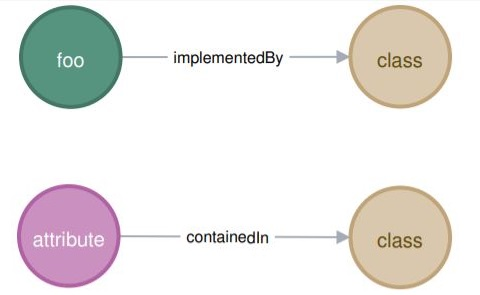
\includegraphics[scale=0.8]{Tesi/Sezione3-RiconoscimentoSmell/immagini/Cattura3.jpg}
                \caption{Esempio di strutture per attributi e funzioni}
            \end{figure}    


\newpage
\section{Riconoscimento di nuovi architectural smell con Arcan}

%Introduzione
Obiettivo di questo capitolo è l'introduzione e approfondimento dei tre nuovi \textit{architectural smell (AS)} introdotti. Le sezioni successive sono orientate alla descrizione dei tre nuovi \textit{smell}, rappresentati secondo una struttura ben definita:
\begin{enumerate}
    \item Introduzione con descrizione delle cause più comuni che portano al suo inserimento nel sistema e piccola descrizione del nodo introdotto nel grafo
    \item Impatto sulla qualità del codice e possibili strategie di \textit{refactoring}
    \item Strategie di identificazione ideate
    \item Algoritmo di \textit{detection} in pseudocodice
\end{enumerate}
Per favorire la comprensione degli \textit{smell} è necessaria l'introduzione del concetto di \textit{abstraction}, riferito a classi (concrete o astratte) e interfacce che fanno parte del progetto. Questo termine deriva dal \textit{Abstraction Principle} \cite{booch2008object}, che sostiene la semplificazione delle entità attraverso l'eliminazione di dettagli non necessari e la generalizzazione delle caratteristiche condivise tra esse. Un altro principio importante per la comprensione del lavoro svolto è il \textit{Hierarchy Principle} \cite{booch2008object}, che supporta la creazione di un'organizzazione gerarchica di \textit{abstraction} attraverso l'utilizzo di tecniche come classificazione, generalizzazione e sostituibilità.

Obiettivo dell'estensione di Arcan è stato fornire al \textit{tool} la capacità di riconoscere tre nuovi \textit{architectural smells}: \textit{Subclasses Do Not Redefine Methods}, \textit{Unutilizied Abstraction}, e \textit{Unnecessary Abstraction}. 
%In dettaglio, i nuovi smell introdotti sono:
Tutti gli \textit{smell} introdotti violano i principi presentati in precedenza. In dettaglio, lo smell \textit{Subclasses Do Not Redefine Methods} è responsabile della violazione del \textit{Hierarchy Principle} mentre \textit{Unutilizied Abstraction} e \textit{Unnecessary Abstraction} non rispettano il \textit{Abstraction Principle}.


%\input{Tesi/Sezione3-RiconoscimentoSmell/subfiles/3.1_Arcan_e_modifiche}

\subsection{Subclasses Do Not Redefine Methods}
    \textit{Subclasses Do Not Redefine Methods} (\textit{SR}), definito da M. Lippert et al. \cite{lippert2006refactoring}, afferma che se le sottoclassi non ridefiniscono i metodi delle loro superclassi può essere indice del fatto che attraverso l'ereditarietà non è espressa nessuna astrazione ma è più che altro ereditarietà implementativa \cite{lippert2006refactoring}.
        %è uno \textit{smell} definito da M. Lippert e S. Roock \cite{lippert2006refactoring} \cite{SURYANARAYANA201521} che si verifica quando una sottoclasse non ridefinisce nessun metodo della sua superclasse. 
        
    Questo può essere indice del fatto che attraverso la gerarchia non è espressa nessuna astrazione e che non c'è quindi alcun motivo per cui questa gerarchia debba essere presente nel design. 
    La presenza di questo \textit{smell} può essere causata principalmente dalla tendenza all'utilizzo delle gerarchie per il riutilizzo delle funzionalità del padre, senza però che la classe e il suo supertipo condividano una relazione IS-A. 
    
    \paragraph{Nodo di tipo smell nel grafo}
    Il nodo dello \textit{smell} SR dispone di due o più archi in uscita verso altrettante \textit{unit}: 
    \begin{itemize}
        \item Presenta la dipendenza \textit{affects} verso la \textit{unit} colpita dallo \textit{smell}.
        
        \item È in relazione con almeno una \textit{unit} attraverso un arco di tipo \textit{fatherInvolved}, che indica i supertipi della classe che presenta lo \textit{smell}.
    \end{itemize}
    
    %Problemi e refactoring
    \subsubsection{Impatto sulla qualità del codice e refactoring}
        %La presenza di questo smell può influenzare diversi aspetti riguardanti la qualità del codice \cite{SURYANARAYANA201521}, come  comprensibilità, riusabilità, facilità nella modifica ed estensione, affidabilità sono tutti affetti negativamente dalla presenza di \textit{Subclasses Do Not Redefine Methods}. 
        La presenza di \textit{Subclasses Do Not Redefine Methods} può influenzare in maniera negativa la qualità del codice attraverso la compromissione di proprietà quali comprensibilità, riusabilità, facilità nella modifica, estensione e affidabilità \cite{SURYANARAYANA201521}.
        
        Analizzando nel dettaglio le qualità influenzate negativamente dalla presenza di questo \textit{smell}, si può affermare che:
        \begin{itemize}
            \item Quando le classi in una relazione gerarchica non condividono una relazione concettuale IS-A, può portare a molta confusione e ridurre la \textit{comprensibilità} del sistema, confondendo gli sviluppatori e i progettisti.
            
            \item Se le \textit{unit} non condividono una relazione IS-A il riutilizzo del codice potrebbe essere compromesso poiché non è possibile la sostituzione delle istanze dei sottotipi con i loro supertipi. Questa situazione renderebbe difficile il \textit{riutilizzo} dell'intera gerarchia in un altro contesto. Questo potrebbe causare diversi problemi ulteriori relativi alla difficoltà nella \textit{modifica ed estensione} della gerarchia, poiché un cambiamento potrebbe avere un grosso impatto sul codice.
            
            \item La presenza di classi che non condividono una relazione IS-A potrebbe portare a diversi problemi di \textit{affidabilità} del codice, poiché lo scambio tra un'istanza di una superclasse con quella di una sottoclasse potrebbe causare errori indesiderati.
        \end{itemize}
        
        Per il \textit{refactoring} di questo \textit{smell} l'applicazione di \textit{Replace Inheritance With Delegation} è la scelta consigliata e più diffusa \cite{SURYANARAYANA201521}. Questa strategia consiste nella trasformazione della relazione IS-A tra le due classi in una relazione di utilizzo, in modo che la ex-sottoclasse abbia al suo interno un oggetto dell'altra per l'utilizzo dei suoi metodi.
        
        % Considerazioni sullo smell (esempio cosa dell'overloading - già approfondita sopra - , )
    
    %Strategie di identificazione
    \subsubsection{Strategia di identificazione}
        Devo controllare che in ogni relazione gerarchica presente nel programma analizzato non si verifichi la ridefinizione di almeno un metodo del supertipo da parte del sottotipo. Per fare questo, è necessario controllare che l'intersezione dei metodi definiti dalle due classi sia vuota e quindi non abbiano almeno un metodo in comune. 
        Nella ricerca dei metodi definiti dalla superclasse viene utilizzata la funzione \textit{getAllMethods} definita in precedenza poiché, se i metodi delle interfacce non fossero considerati, una situazione analoga a quella definita dalla figura 2, dove il sottotipo (nodo beige) ridefinisce un metodo (nodo verde) definito solamente dall'interfaccia (nodo azzurro) ma non implementato dalla classe astratta (nodo rosso), verrebbe considerata come \textit{smell}. È stato deciso però di non ritenere questa situazione come tale poiché le due classi condividono una relazione IS-A e il metodo dell'interfaccia che la classe concreta implementa è derivato comunque dal suo supertipo.
        %i metodi che la classe astratta può anche non implementare sono stati considerati come fossero \textit{abstract}, ridefiniti poi dalle classi concrete che la estendono.
        \defaultvspace
        \begin{figure}[h]
            \centering
            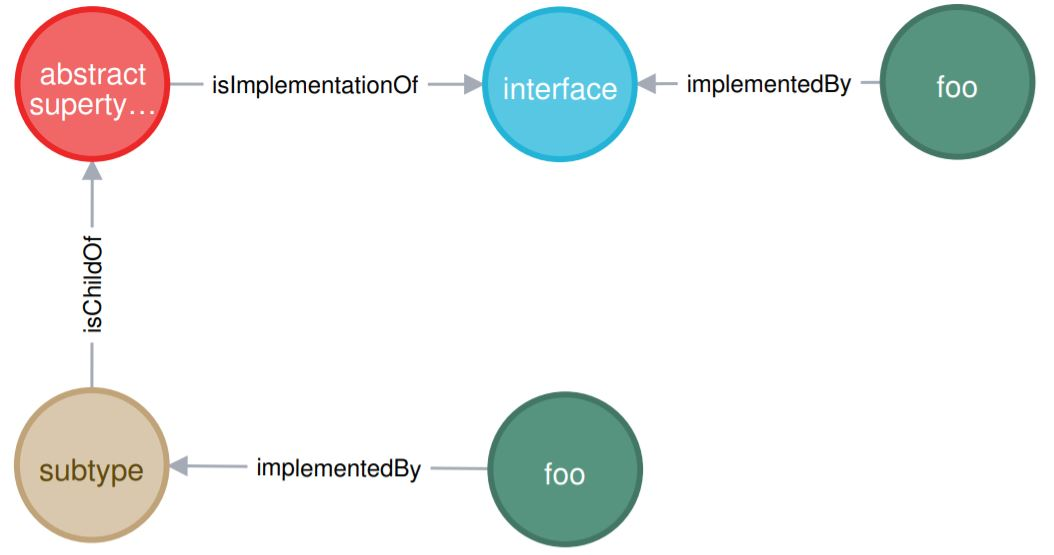
\includegraphics[scale=0.5]{Tesi/Sezione3-RiconoscimentoSmell/immagini/grafo1.JPG}
            \caption{Esempio interfaccia implementata da una classe astratta}
            \label{fig:my_label}
        \end{figure}
        \defaultvspace \\
        %Dalle relazioni considerate vengono escluse però quelle gerarchiche tra due interfacce, p
        %Per l'identificazione di questo smell inoltre non sono state considerate due diverse categorie di unit:
        Dalle relazione \textit{isChildOf} considerate vengono escluse tutte quelle che coinvolgono:
        \begin{itemize}
            \item Due \textit{unit} \textit{interface}, poichè nelle gerarchie tra interfacce non avviene la ridefinizione di metodi ma si verifica solamente l'estensione del comportamento attraverso nuove funzioni, pertanto tutti questi casi risulterebbero falsi positivi.
            
            \item Una \textit{unit} di tipo classe che rappresenta una \textit{exception} (oppure anche \textit{error}), poiché è molto comune che abbiano come supertipo una \textit{exception} e richiamino solamente il costruttore utilizzando parametri diversi. In questi casi non c'è ridefinizione dei metodi ma non è stato giudicato comunque come \textit{smell}, in quanto la relazione IS-A è presente.
        \end{itemize}
        %
        % tutte le coppie di nodi di tipo classe che condividono una relazione \textit{isChildOf} dove
        In termini di grafo è necessario considerare tutti i nodi che presentano un arco \textit{isChildOf} in uscita dove almeno un nodo di tipo \textit{function} in ingresso al nodo considerato non condivida la proprietà \textit{name} con un'altro nodo \textit{function}:
        \begin{itemize}
            \item Definito da uno dei supertipi della classe analizzata, dove per supertipi si intendono i nodi che hanno in ingresso gli archi \textit{isChildOf} provenienti dalla classe sotto analisi.
            
            \item Presente nella gerarchia di uno dei supertipi. Per verificare questo si seguono tutti gli archi \textit{isChildOf} e \textit{implementedBy} a partire dai supertipi al fine di controllare anche tutti i metodi ereditati.
        \end{itemize}
        %In termini di grafo bisogna considerare tutte le coppie di nodi di tipo classe che condividono una relazione isChildOf dove il nodo del supertipo non ha in ingresso un nodo function che condivide il nome con almeno un nodo function che la unit padre ha in ingresso. 
        %Inoltre è necessario risalire la gerarchia seguendo le relazioni \textit{isChildOf} per verificare che il sottotipo non abbia un nodo function 
        %Inoltre è necessario anche risalire la gerarchia della classe padre per verificare che il sottotipo non ridefinisca qualche metodo che il padre erediti dalla sua gerarchia, poichè il parser delle funzioni non include nella unit eventuali metodi ereditati. DA MIGLIORARE LE InFo sUL GRAFO
        
    
    %Algoritmo
    \subsubsection{Algoritmo}
        \paragraph{Input} un sottografo del grafo principale, considerando solamente i nodi che rappresentano classi (concrete e astratte) coinvolte in una dipendenza del tipo \textit{isChildOf} e le relative funzioni definite dalle classi. Oltre all'arco \textit{isChildOf} sarà considerato anche \textit{implementedBy}.
        %Gli archi considerati sono invece di tipo \textit{isChildOf} e \textit{implementedBy}
    
        \paragraph{Output} una lista di classi che presentano lo \textit{smell} e i relativi supertipi coinvolti.
        
        \paragraph{Algoritmo}
            \begin{algorithmic}
    \Function{Subclasses-does-not-redefine-methods-detector}{ }
        \State{Prendo tutti i nodi che hanno almeno un arco in entrata del tipo}
        \State{isChildOf, escludendo le interfacce e le enumerazioni}
        \For{Ogni vertice trovato, che rappresenta il supertipo}
            \State{Prendo la lista delle funzioni definite ed ereditate dalla unit,}
            \State{includendo anche quelli definiti dalle interfacce implementate}
            \If{La lista dei metodi considerata non è vuota}
                \For{Ogni sottotipo con isChildOf in uscita verso il supertipo}
                    \State{Prendo la lista di tutte le funzioni definite dal sottotipo}
                    \If{L'intersezione tra le liste dei metodi è l'insieme vuoto}
                        \State{Aggiungo il vertice alla lista degli smell}
                    \EndIf
                \EndFor
             \EndIf
        \EndFor
    \EndFunction
\end{algorithmic}
    


\subsection{Unutilizied Abstraction}
    \textit{Unutilizied Abstraction} (\textit{UUA}), definito da G. Suryanarayana et al. \cite{SURYANARAYANA201521}, si manifesta quando una \textit{abstraction} viene lasciata inutilizzata, cioè non direttamente usata o non raggiungibile. Questo \textit{smell} si può manifestare in due forme: 
        \begin{itemize}
        \item \textit{Unreferenced Abstraction}, classi concrete che non sono utilizzate da nessuno.
        
        \item \textit{Orphan Abstraction}, classi astratte e interfacce che non hanno nessuna abstraction derivata.
    \end{itemize}
    %
    Il principio di astrazione afferma che le \textit{abstraction} dovrebbero avere loro assegnate responsabilità singole e limitate. La presenza di classi e interfacce senza uno scopo specifico nel design e quindi inutilizzate viola il principio, introducendo nel design questo \textit{smell}. Un altro principio violato oltre a quello di astrazione è il principio \textit{YAGNI (You Aren't Gonna Need It} \cite{yagniFowler}, che raccomanda di evitare l'aggiunta di funzionalità non strettamente necessarie al design.

    Le cause che possono portare all'introduzione di \textit{UNA} nel design sono:
    \begin{itemize} %Sicuramente sistemare la forma - 
        \item \textit{Design speculativo}: l'introduzione nel design di funzionalità e strutture che potrebbero servire in futuro può portare alla violazione del principio \textit{YAGNI} \cite{yagniFowler} e all'introduzione di \textit{abstraction} attualmente non utilizzate.
            %una condizione che si verifica quando i progettisti introducono nel design funzionalità e strutture che potrebbero servire in futuro, violando il principio You Aren't Gonna Need It \cite{yagniFowler}.
            % la tendenza allo sviluppo orientata al futuro è una condizione che si verifica quando
        
        \item \textit{Cambio di Requisiti}: il cambiamento di requisiti del progetto potrebbe avere influenza anche sulle \textit{abstraction} impiegate, perciò alcune potrebbero rimanere orfane e non utilizzate.
            %non è anomalo che durante lo sviluppo di un nuovo sistema i requisiti dello stesso cambino in continuazione, portando agli sviluppatori una continua attività di modifiche e cambi al progetto; proprio per questo motivo, sono stati introdotti i metodi agili \cite{checosa?}. Questi continui cambi di requisiti hanno effetto sulle funzionalità e soprattutto sulle abstraction utilizzate del progetto, che potrebbero quindi non essere più utilizzate e rimanere orfane nel design.
        
        \item \textit{Cancellazione parziale delle abstraction}: quando la \textit{manutenzione} di un progetto viene effettuata senza cancellare \textit{abstraction} vecchie e non più utili per il design, lasciando così nel sistema diverse \textit{unutilizied abstraction}.
            % durante la manutenzione di un progetto, si effettuano diverse attività tra cui appunto la cancellazione delle abstraction non più attive. Se quest'ultima attività viene effettuata parzialmente o non viene proprio svolta, potrebbero rimanere nel progetto abstraction vecchie e che non servono più al design, lasciando così nel sistema diverse Unutilized Abstraction.
        
        \item \textit{Paura di rompere il codice}: la cancellazione di \textit{abstraction} potrebbe portare diversi problemi ai programmatori poiché spesso essi decidono di non rimuoverle per paura che vengano ancora utilizzate nel codice. L'introduzione dello \textit{smell} causata da questo timore si verifica soprattutto in progetti che presentano un grande numero di classi e linee di codice.
        %quando non viene effettuata la cancellazione di abstraction poichè i programmatori hanno paura che quella classe sia ancora utilizzata da qualche parte nel codice e che quindi la loro cancellazione possa portare svariati problemi. Questa condizione si verifica soprattutto in grandi progetti con molte classi e loc.
    \end{itemize}
    
    \paragraph{Nodo di tipo smell nel grafo}
        Il nodo dello \textit{smell} UUA si presenta come un nodo di tipo \textit{smell} con una singola dipendenza verso la classe che presenta il problema.
    
    
    %Impatto
     \subsubsection{Impatto sulla qualità del codice e refactoring}
         \textit{Unutilizied Abstraction} ha un impatto fortemente negativo su due qualità del progetto, ovvero affidabilità e facilità di comprensione del sistema. La presenza di molte classi inutilizzate infatti potrebbe portare ad errori a run-time, se per esempio una di queste dovesse venire erroneamente invocata portandosi dietro piccoli \textit{bug}. Inoltre l'inquinamento del design da parte di molte classi e interfacce diminuisce la comprensione del progetto aumentandone il carico cognitivo, causando anche problemi secondari come difficoltà nello studio del funzionamento del sistema oppure estensione e manutenzione del codice complicate.
         %e può portare a diversi problemi secondari come difficoltà a studiare il funzionamento del prodotto oppure problemi con l'estensione o la manutenzione del codice.
        
        La tecnica di \textit{refactoring} consigliata è l'eliminazione del progetto di tutte le \textit{abstraction} non più necessarie. Nel caso di API pubbliche però l'eliminazione potrebbe non essere la soluzione opportuna, poiché alcune di esse potrebbero ancora essere utilizzate da qualche \textit{client}. La soluzione in questo caso è la segnalazione delle \textit{unutilizied abstraction} come deprecate.
        % Nel caso di API pubbliche che possono essere ancora utilizzate da qualche client invece, è opportuno segnalare come deprecate le abstraction coinvolte.

    %Problemi
    
    %Considerazioni fatte sullo smell (Esempio la cosa dell'overloading per SR)
    
    %Strategie di identificazione
    \subsubsection{Strategie di identificazione}
        Per l'identificazione dello \textit{smell} \textit{Unutilizied Abstraction} è necessaria l'identificazione di tutte le \textit{abstraction} del progetto inutilizzate oppure non utilizzate per il loro naturale scopo. In particolare, come già analizzato nella sua introduzione, bisogna considerare tutte quelle che appartengono a due differenti categorie:
        \begin{itemize}
            \item \textit{Unreferenced Abstractions}, classi concrete non utilizzate da nessuno e senza alcun riferimento all'interno del progetto, interpretato nel grafo come i nodi che non presentano in ingresso alcun arco \textit{dependsOn} proveniente da una classe esterna.
            Quest'ultima precisazione viene specificata poiché nel grafo di Arcan le \textit{inner class} hanno sempre una relazione \textit{dependsOn} verso il loro contenitore e, senza questa specificazione, le classi \textit{unreferenced} contenenti almeno una classe interna non utilizzata non sarebbero state erroneamente considerate come \textit{smell}. 
            L'utilizzo di una classe interna da parte di una esterna genera invece nel grafo due differenti archi \textit{dependsOn}, uno in ingresso alla classe utilizzata e l'altro a quella che la contiene. In questo caso, anche se la classe contenitore non viene utilizzata, non viene giustamente considerato come \textit{smell}.  
            
            \item \textit{Orphan Abstractions}, classi astratte o interfacce che non vengono implementate o estese. Per quanto riguarda le classi astratte, bisogna ricercare nel grafo tutti i nodi che le rappresentano senza nessun arco \textit{isChildOf} in ingresso; i nodi di tipo interfaccia invece non devono presentare in ingresso, oltre ad archi \textit{isChildOf}, nemmeno nessuna relazione di tipo \textit{isImplementationOf}.
            %, ovvero nodi del grafo di tipo classe astratta e interfaccia che non presentano nessun arco di tipo \textit{isChildOf} in ingresso, oppure nodi interfaccia che non presentano archi \textit{isImplementationOf} in ingresso. 
            In questo caso non si deve porre molta attenzione alle classi interne, poiché per la \textit{detection} di questo caso non vengono presi in considerazione gli archi del tipo dependsOn.
        \end{itemize}
        
    \subsubsection{Algoritmo}
        \paragraph{Input} un sottografo del grafo principale considerando solamente i nodi che rappresentano classi e interfacce e gli archi \textit{isChildOf}, \textit{dependsOn} oppure \textit{isImplementationOf}. 
        
        \paragraph{Output} una lista di unit che presentano lo \textit{smell}.
        
        \paragraph{Algoritmo}
        \begin{algorithmic}
\Function{unutilizied-abstraction-detector}{}
\State{Prendo la lista di tutti i nodi unit}
\For{Ogni vertice della lista}
    \If{Il vertice è di tipo classe o enum}
        \State{Considero tutti i nodi con un arco dependsOn in uscita verso}
        \State{il vertice}
    \EndIf
    \If{Il vertice è di tipo classe astratta}
        \State{Considero tutti i nodi con un arco isChildOf verso il vertice}
    \EndIf
    \If{Il vertice è di tipo interfaccia}
        \State{Considero tutti i nodi con un arco dependsOn oppure }
        \State{isChildOf verso il vertice}
    \EndIf
    
    \If{I nodi considerati sono 0 oppure sono tutti classi interne}
        \State{Aggiungi il nodo alla lista degli smell}
    \EndIf
    
\EndFor
\EndFunction 
\end{algorithmic}


    

\subsection{Unnecessary Abstraction}
    \textit{Unnecessary Abstraction} (\textit{UNA}), definito da G. Suryanarayana et al. \cite{SURYANARAYANA201521}, si verifica quando un \textit{abstraction} che non è in realtà necessaria (e quindi potrebbe essere evitata) viene introdotta nel design.
    Questo \textit{smell} viola il principio di astrazione, poiché si verifica l'introduzione nel design di \textit{abstraction} con responsabilità limitate oppure nulle.
    
    Si possono riassumere tre cause principali che portano l'introduzione di questo \textit{smell} nel design:
        %Le cause principali dell'introduzione di questo \textit{smell} nel sistema si possono riassumere in tre differenti casi:
    \begin{itemize}
        \item \textit{Utilizzo improprio di feature del linguaggio:}
        \textit{abstraction} non necessarie possono essere introdotte nel design solamente per convenienza, utilizzando \textit{feature} del linguaggio in maniera impropria. Il caso più diffuso è rappresentato dalle \textit{constant placeholder}, interfacce o classi utilizzate dal programmatore solamente per contenere valori costanti.
        La generazione di queste \textit{abstraction} consente al programmatore di implementare o estendere il \textit{placeholder} nella classe desiderata in modo da utilizzare una costante senza la necessità di specificarne il tipo ma solamente attraverso il suo nome.
        
        \item \textit{Over-engineering:} vengono definite \textit{over engineered} le \textit{abstraction} introdotte nel design che risultano superflue e prive di un grande significato associato. 
        Un esempio di classe over engineered è mostrato dalla figura 3, dove sono presenti una classe \textit{Customer} contenente un attributo ID che, invece di essere di tipo \textit{String}, è incapsulato da una classe \textit{CustomerID} dedicata, superflua e non necessaria per il sistema.
        %Un esempio di questo caso può essere rappresentato da una classe Customer contenente un attributo CustomerID che, al posto di essere un attributo \textit{String} di Customer, ha una classe CustomerID dedicata che presenta getter e setter, costruttore e appunto un parametro ID di tipo \textit{String}. CustomerID risulta quindi superflua e non necessaria per il sistema.
        \begin{figure}[h]
            \centering
            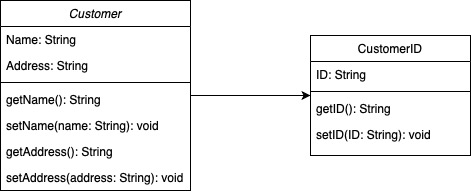
\includegraphics[scale=0.45]{Tesi/Sezione3-RiconoscimentoSmell/immagini/Untitled Diagram.jpg}
            \caption{Esempio di classe over engineered}
            \label{fig:my_label}
        \end{figure}
        
        
        \item \textit{Procedural thinking:} %si verifica quando lo sviluppatore, soprattutto se sè è affacciato di recente allo sviluppo object-oriented, tende a pensare le classi in modo procedurale.
        se uno sviluppatore, spesso affacciato recentemente allo sviluppo Object Oriented, tende a pensare le classi in maniera procedurale e non dotate di responsabilità e compiti, può introdurre nel codice \textit{abstraction} non necessarie. 
        Questa tendenza si traduce in classi che "svolgono procedure" invece di "essere qualcosa" violando il principio di astrazione, a causa di responsabilità multiple e poco definite. Un esempio di classe procedurale possono essere le classi di \textit{utilities}.
    \end{itemize}
    
    
    \paragraph{Nodo di tipo smell nel grafo}
        Il nodo dello \textit{smell} presenta un'unica dipendenza verso la sospetta \textit{Unnecessary Abstraction}. Inoltre ha una proprietà chiamata \textit{unnecessaryCase}, che indica quale delle tre casistiche di \textit{UNA} è stata riscontrata nella \textit{unit}.
        
            
    %Problemi e refactoring
    \subsubsection{Impatto sulla qualità del codice e refactoring}
        \textit{Unnecessary Abstraction} ha un impatto significativo sulla possibilità di riutilizzo del codice e sulla comprensione del progetto. 
        Riguardo la comprensione, la presenza di numerose interfacce non necessarie incide in maniera negativa poiché aumenta la complessità del design, causando una maggiore difficoltà nell'interpretazione del design e nella chiarezza del progetto.
        
        Anche il riutilizzo del codice subisce un influenza negativa dalla presenza di \textit{Unnecessary Abstraction} poiché \textit{abstraction} senza responsabilità uniche e ben definite e specializzate per un design particolare risultano molto difficili da riutilizzare in contesti differenti.
        
        Se inoltre viene utilizzata un'interfaccia come \textit{constant placeholder} possono verificarsi ulteriori problemi:
        \begin{itemize}
            \item Le classi derivate da quelle che implementano l'interfaccia possono risultare inquinate da costanti che non sono rilevanti per loro.
            
            \item Si verifica una violazione dell'incapsulamento in quanto vengono mostrati, attraverso l'interfaccia, dettagli implementativi.
            
            \item Quando le costanti sono presenti nelle interfacce, cambiamenti ad esse possono creare problemi ai \textit{client} esistenti.
            
            \item Le interfacce rappresentano un protocollo che le classi che lo implementano devono rispettare e l'utilizzo come \textit{constant placeholder} è un abuso del meccanismo di astrazione.
        \end{itemize}
        
        Al fine di rimuovere questo problema dal codice ed aumentare la qualità dello stesso, sono suggerite tre diverse strategie \cite{SURYANARAYANA201521} di \textit{refactoring}:
        \begin{itemize}
            \item Le classi procedurali dovrebbero essere eliminate, secondo quanto proposto da Fowler \cite{fowler2018refactoring}.
            
            \item Si suggerisce l'eliminazione delle \textit{constant placeholder} per favorire l'utilizzo di costrutti forniti dal linguaggio che si adattano meglio a questa esigenza (un esempio possono essere le enumerazioni).
            
            \item Per le classi \textit{over engineered} Fowler consiglia \cite{fowler2018refactoring} l'applicazione del \textit{Inline Class Refactoring}, che consiste nell'unione delle due classi in una sola. Riferendoci all'esempio presentato in precedenza, l'azione suggerita è l'aggiunta di un parametro \textit{CustomerID} di tipo \textit{String} alla classe \textit{Customer}, eliminando la classe \textit{CustomerID} non necessaria.
        \end{itemize}
        
    
    %Considerazioni fatte sullo smell (Esempio la cosa dell'overloading)
    
    %Strategie di identificazione
    \subsubsection{Strategia di identificazione}
        Le regole di identificazione di \textit{Unnecessary Abstraction} sono state divise in tre differenti casistiche, in base alle cause della presenza di questo \textit{smell} definite nella sezione 4.3. Vengono considerate per la valutazione della presenza di \textit{UNA}:
        \begin{itemize}
            \item \textit{Placeholder abstraction} classi oppure interfacce senza alcuna funzione definita al loro interno che contengono solamente attributi costanti. La ricerca di queste classi ha visto l'esclusione di due categorie principali di \textit{unit}, in quanto risultanti come falsi positivi. Non sono state considerate le enumerazioni, poiché sono per definizione contenitori di costanti, e tutte le classi \textit{exception} o \textit{error}, poiché anche se presentano le caratteristiche delle \textit{constant placeholder} non possono essere considerate come tali. Sono state escluse inoltre tutte le classi che presentano un supertipo, con le uniche eccezioni di  padri vuoti oppure contenenti solamente costanti.
            
            Nel grafo le \textit{placeholder abstraction} vengono rappresentate da tutti i nodi senza archi in ingresso di tipo \textit{implementedBy} e, per ogni arco in ingresso del tipo \textit{definedBy}, il nodo corrispondente all'attributo deve avere i parametri \textit{constantAttribute} e \textit{defaultValue} aventi il valore \textit{true}.
            Vengono esclusi dalla ricerca tutti i nodi \textit{unit} che presentano \textit{componentType} con valore \textit{enum} oppure con nomi che terminano con le stringhe \textit{"Error"} oppure \textit{"Exception"}. Inoltre per le \textit{unit} che presentano  archi \textit{isChildOf} in uscita viene controllato che i supertipi non presentino alcun arco in ingresso oppure che presentino le stesse caratteristiche definite in precedenza.
        
            
            \item \textit{Over-engineered} classi concrete che definiscono solamente un attributo e due funzioni, rappresentanti i metodi \textit{getter} e \textit{setter}. Inoltre queste classi devono essere definite come attributo in solamente un'altra \textit{abstraction} e non possono presentare alcun supertipo che non sia vuoto, poiché altrimenti la classe subirebbe una modifica a causa degli elementi ereditati. Per la definizione di queste regole si è replicato il caso descritto dalla figura 3. È stato deciso inoltre di inserire il limite di solamente un utilizzo come parametro da un'altra \textit{abstraction} poiché altrimenti la classe potrebbe avere significato nel sistema di riferimento, come avviene ad esempio nell'applicazione del pattern \textit{Object Identifier} \cite{brown1996pattern}. 
            
            Le condizioni per l'identificazione si traducono nella ricerca di nodi del grafo che presentano in ingresso un solo arco di tipo \textit{definedBy} e massimo due \textit{implementedBy}. Viene controllato anche che il nome di ogni funzione rappresentata dall'arco \textit{implementedBy} sia effettivamente una funzione \textit{getter} o \textit{setter} per l'attributo della classe, ovvero presenti un nome del tipo \{get/set\}\{nomeAttributo\}. Inoltre il nodo deve presentare solamente un arco in ingresso di tipo dependsOn da un'altra \textit{unit}, che a sua volta ha in ingresso un'arco \textit{containedIn} da un attributo dello stesso tipo della classe sotto esame.
            Se infine il nodo presentasse un arco in uscita di tipo \textit{isChildOf}, la \textit{unit} del supertipo non dovrebbe aver alcun arco in ingresso \textit{definedBy} oppure \textit{implementedBy} ed anche eventuali supertipi di questa \textit{unit} non dovrebbero presentare nessun arco di queste due tipologie. Un esempio di questa struttura può essere osservato nella figura 4 (dove alla classe Customer è stato aggiunto un ulteriore attributo \textit{name}).
            % Non considerate classi con il parametro final e default 
            
            \begin{figure}[h]
                \centering
                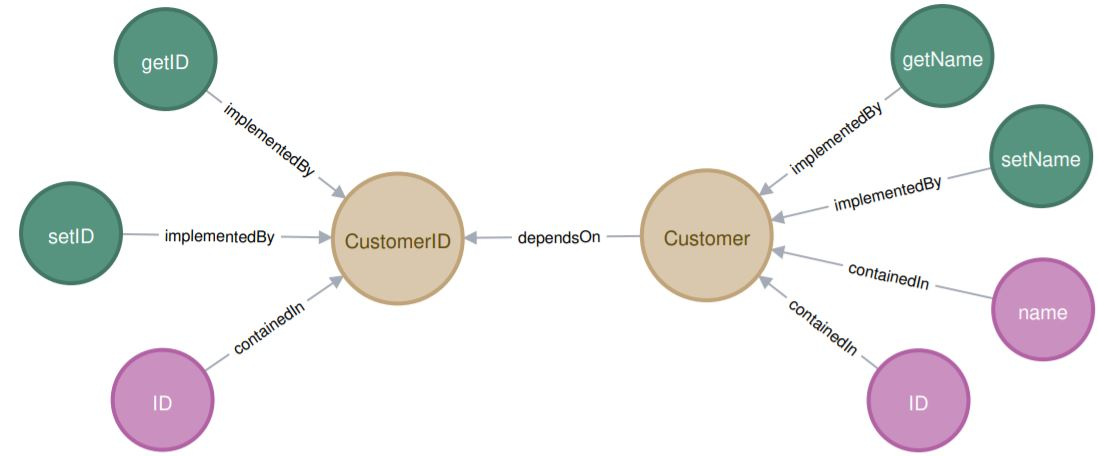
\includegraphics[scale=0.6]{Tesi/Sezione3-RiconoscimentoSmell/immagini/overengineered.JPG}
                \caption{Esempio classi overengineered nel grafo}
                \label{fig:my_label}
            \end{figure}
           
           
           \item \textit{Procedural class} classi concrete o astratte senza attributi e con solamente una oppure due funzioni definite al loro interno. Non sono state considerate nella ricerca tutte quelle classi che presentano dei supertipi, per due motivi principali. In primo luogo, se la classe avesse dei supertipi potrebbe ereditare metodi e attributi che potrebbero far sì che non rispetti più i vincoli appena definiti. Inoltre le classi procedurali sono spesso introdotte da persone non esperte nella programmazione orientata agli oggetti e prive di significato nel design, cosa che potrebbe non verificarsi se è presente una gerarchia.
            
           % Queste strategie si traducono in termini di grafo con tutti 
            Per quanto riguarda il grafo, bisogna ricercare i nodi con \textit{componentType} di valore \textit{class} oppure \textit{abstract\_class} che presentano in ingresso uno oppure due archi di tipo \textit{implementedBy} e nessun arco di tipo \textit{containedIn} in ingresso oppure \textit{isChildOf} in uscita.
        \end{itemize}
        
    %Algoritmo
    \subsubsection{Algoritmo}
        \paragraph{Input} un sottografo del grafo principale, contenente i nodi \textit{unit} e le \textit{function} e \textit{attribute} che esse definiscono. Gli archi considerati sono di tipo \textit{dependsOn}, \textit{implementedBy} e \textit{definedIn}. 
        
        \paragraph{Output} la lista delle classi affette da questo \textit{smell} e la relativa causa che ha portato alla loro identificazione. 
        
        \paragraph{Algoritmo}
            \begin{algorithmic}
    \Function{unnecessary-abstraction-detection}{G}
        \State{Prendo la lista di tutti i vertici di tipo unit}
        \For{Ogni vertice nella lista}
            %Procedural
            \If{\Call{is-procedural-class}{vertice}}
                \State{Aggiungo il vertice alla lista degli smell}
            \EndIf
            %Costant
            \If{\Call{is-constant-placeholder}{vertice}}
                \State{Aggiungo il vertice alla lista degli smell}
            \EndIf
            %Over
            \If{\Call{is-over-engineered}{vertice}}
                \State{Aggiungo il vertice alla lista degli smell}
            \EndIf
        \EndFor
    \EndFunction
    \\
    \Function{is-procedural-class}{vertice}
        \If{Il vertice è una classe concreta o astratta}
            \If{Il vertice non ha archi in ingresso containedIn}
                \If{Il vertice non ha archi in uscita isChildOf}
                    \If{Il vertice ha 1-2 archi in ingresso implementedBy}
                        \State{\textbf{return} la classe è una Unnecessary Abstraction}
                    \EndIf
                \EndIf
            \EndIf
        \EndIf
    \EndFunction
    \\
    \Function{is-constant-placeholder}{vertice}
        \If{Il vertice non rappresenta enumerazioni o classi di errore}
            \If{La classe non ha archi in ingresso implementedBy}
                \If{La classe ha archi in uscita isChildOf}
                    \If{Almeno un supertipo non è una constant placeholder op-\\\hspace{2.3cm}pure non è vuoto}
                        \State{\textbf{return} la classe non è una Unnecessary Abstraction}
                    \EndIf
                \EndIf

                \If{Tutti i nodi con arco containedIn verso questo vertice hanno \\\hspace{1.7cm} gli attributi constantAttribute e defaultValue true}
                    \State{\textbf{return} la classe è una Unnecessary Abstraction}
                \EndIf
            \EndIf
        \EndIf
    \EndFunction
    \\
    \Function{is-over-engineered}{vertice}
        \If{Il vertice ha un solo arco in ingresso containedIn}
            \If{Il vertice ha max 2 archi implementedBy in ingresso con nomi \\\hspace{1.1cm} delle funzioni collegate corrispondono a getNomeAttributo oppure \\\hspace{1.1cm} setNomeAttributo}
                \If{Il vertice ha solo un'arco in ingresso dependsOn da un vertice \\\hspace{1.7cm} che definisce un attributo dello stesso tipo della classe rappresen- \\\hspace{1.7cm}tata dal vertice}
                    \State{\textbf{return} la classe è una Unnecessary Abstraction}
                \EndIf
            \EndIf
        \EndIf
    \EndFunction
\end{algorithmic}

    



\newpage
\section{Riconoscimento degli architectural smell su progetti reali}
    Questo capitolo presenta nel dettaglio tutte le attività svolte riguardanti l'esecuzione e la validazione degli algoritmi sviluppati su diversi progetti open-source. 
    Dopo una descrizione dei progetti, saranno analizzate nel dettaglio l'esecuzione degli algoritmi, le diverse attività di validazione svolte e i risultati ottenuti.  
    %Saranno inoltre approfondite anche tutte le operazioni per la validazione dei risultati, con descrizione delle differenti attività svolte e considerazioni approfondite sugli smell e sulle cause che hanno portato alla detection di falsi positivi. 
    Sarà inoltre effettuato un confronto sulle differenze della \textit{detection} di Arcan rispetto a quella del \textit{tool} Designite \cite{Designite}.
    Un'ultima sezione esporrà poi i differenti problemi affrontati durante lo svolgimento di queste attività.
    Prima della presentazione delle tematiche descritte in precedenza, sarà effettuata una breve digressione riguardo le attività di \textit{testing} svolte per la verifica degli algoritmi durante il loro sviluppo %e la correttezza dei risultati prodotti con input ben definiti. 

    \paragraph{Approccio Test Driven Development}
        Durante lo sviluppo degli algoritmi sono stati effettuati i loro test seguendo l'approccio \textit{Test Driven Development (TDD)} \cite{beck2003testdrivendev}. Questa strategia prevede la scrittura dei test anticipata rispetto all'implementazione degli algoritmi, in modo che lo sviluppo dell'applicativo sia orientato alla soddisfazione degli stessi. Al fine di applicare il \textit{TDD} è stato utilizzato il framework JUnit \cite{JunitWebsite}.
            % Inizialmente la prima fase di testing della capacità e correttezza degli algoritmi è stata durante lo sviluppo degli stessi, mediante l'utilizzo del framework JUnit \cite{JunitWebsite} per la creazione di test unitari. E' stato scelto infatti un approccio di Test Driven Development (TDD) \cite{beck2003testdrivendev}, che prevede la scrittura dei test prima dell'implementazione degli algoritmi in modo che lo sviluppo dell'applicativo abbia come obiettivo il passaggio di tutti i test unitari. 
        
        L'implementazione dei test unitari è stata fondamentale per la definizione degli obiettivi da raggiungere da parte degli algoritmi di \textit{detection}. Attraverso queste verifiche è stato possibile effettuare due tipologie di analisi differenti:
        \begin{itemize}
            \item \textit{Analisi di strutture sintetiche}, cioè grafi generati manualmente all'interno del codice dei test, utilizzati al fine di valutare il comportamento dell'algoritmo considerate diverse situazioni in termini di nodi e relazioni tra essi. In particolare attraverso le strutture sintetiche sono stati analizzati tutti i casi limite riguardanti le strutture del grafo, come ad esempio il numero di nodi coinvolti oppure le loro tipologie. L'obiettivo della scrittura di questi test è stato quindi il test su piccola scala, testando la capacità dell'algoritmo a riconoscere gli \textit{smell} in differenti scenari con un numero basso di nodi e archi e strutture ben definite.
            
            \item \textit{Analisi di piccoli progetti open source}, sono stati direttamente analizzati anche due progetti Java \textit{open source} di piccole dimensioni, Junit 4.13 \cite{JunitWebsite} e Jsoniter \cite{JsoniterWebsite}. Lo scopo dell'analisi di questi due progetti è stata la verifica, direttamente dal grafo generato da Arcan tramite la piattaforma Neo4J \cite{Neo4JWebsite}, che il numero degli \textit{smell} trovati attraverso \textit{query} Cypher \cite{Cypher} effettuate sul grafo fosse equivalente a quello trovato dagli algoritmi di \textit{detection}. Questi test quindi avevano come obiettivo la verifica che le strutture sintetiche riconosciute dall'algoritmo fossero individuate anche all'interno di progetti complessi e organizzati.
        \end{itemize}


    \subsection{Descrizione progetti utilizzati}
        Per le attività di individuazione degli \textit{smell} e validazione del lavoro svolto sono stati selezionati dieci progetti \textit{open-source} differenti, sviluppati da \textit{Apache Software Foundation} \cite{apache} e disponibili sulla piattaforma \textit{GitHub} \cite{github}. Una descrizione sommaria dei progetti è fornita dalla tabella 1, presentando informazioni riguardanti numero della release analizzata, dominio applicativo e collegamento al progetto disponibile su \textit{Github}.

A causa di alcuni problemi derivati dalle librerie utilizzate per il \textit{parsing} non è stato possibile analizzare tutti e dieci i progetti completi in tutti i loro componenti, perciò per alcuni di essi è stata necessaria l'analisi solamente del modulo principale del sistema. Nello specifico, per i progetti \textit{Druid}, \textit{Flink} e \textit{Geode} è stato utilizzato il modulo \textit{core} mentre per \textit{Beam} il modulo \textit{beam-runners core-java}.
Per l'analisi inoltre sono state escluse tutte le classi di test, in quanto considerate non molto significative ai fini del lavoro di ricerca degli \textit{smell} e loro validazione.

Informazioni più dettagliate sui progetti riguardanti modulo analizzato, righe di codice (\textit{LOC}) e numero di unit e package analizzati sono verificabili nella tabella 2. \\

% TABELLA DESCRIZIONE
\begin{table}[h]
    \centering
    \begin{tabular}{|c|c|c|c|c|}
        \hline
        \textbf{Progetto} & \textbf{Link} & \textbf{Release} & \textbf{Dominio applicativo}  \\
        \hline
        Accumulo & \cite{accumulogithub} & 2.0.0 & Distributed key/value data store  \\
        %\hline
        Beam & \cite{beamgithub} & 2.20.0 & Unified programming model  \\
        %\hline
        Bookkeeper & \cite{bookkeepergithub} & 4.10.0 & Storage service  \\
        %\hline
        Cassandra & \cite{cassandragithub} & 3.11.6 & Distributed NoSQL DBMS  \\
        %\hline
        Druid & \cite{druidgithub} & 0.18.0 & Distributed data store  \\
        %\hline
        Flink & \cite{flinkgithub} & 1.10.0 & Distributed processing engine  \\
        %\hline
        Geode & \cite{geodegithub} & 1.12.0 & In-memory data management system  \\
        %\hline
        Kafka & \cite{kafkagithub} & 2.5.0 & Distributed platform  \\
        %\hline
        Skywalking & \cite{skywalkinggithub} & 7.0.0 & Application performance monitor system  \\
        %\hline
        Zookeeper & \cite{zookeepergithub} & 3.6.0 & Services for distributed system  \\
        \hline
    \end{tabular}
    \caption{Informazioni progetti analizzati}
    \label{tab:caption}
\end{table}
\defaultvspace
\begin{table}[h]
    \centering
    \begin{tabular}{|c|c|c|c|c|c|}
        \hline
        \textbf{Progetto} & \textbf{Modulo} & \textbf{N\textsuperscript{o} classi} & \textbf{N\textsuperscript{o} package} & \textbf{N\textsuperscript{o} LOC}  \\
        \hline
        Accumulo & - & 3 789 & 212 & 43 682 818 \\
        Beam & core-java & 201 & 8 & 52 414 \\
        Bookkeeper & - & 2 036 & 252 & 1 495 659 \\
        Cassandra & - & 3 910 & 116 & 33 968 645 \\
        Druid & druid-core & 736 & 63 & 369 487 \\
        Flink & flink-core & 915 & 49 & 148 600 \\
        Geode & geode-core & 4 293 & 190 & 2 236 679\\
        Kafka & - & 2 389 & 138 & 575 967 \\
        Skywalking & - & 979 & 526 & 141 674 \\
        Zookeeper & - & 755 & 52 & 269 378 \\
        \hline
    \end{tabular}
    \caption{Dettaglio progetti analizzati}
    \label{tab:caption}
\end{table}


    \subsection{Risultati della detection}
        L'analisi dei progetti è stata effettuata attraverso l'esecuzione di Arcan, in grado di generare in \textit{output} diversi file in formato \textit{csv} per ogni sistema analizzato. I file generati per un singolo progetto forniscono informazioni riguardanti:
\begin{itemize}
    \item I valori delle metriche (come \textit{instability, LOC}) calcolate su tutti gli elementi presenti nell'applicativo.
    
    \item Le unit colpite dallo \textit{smell} (con relazione \textit{affects} verso il nodo che lo rappresenta) e la tipologia riscontrata.
    
    \item Tutte le unit collegate ad un nodo di tipo \textit{smell}, con indicazione sulla tipologia di relazione tra i due elementi.
\end{itemize}
L'analisi di questi tre \textit{file} ha permesso lo studio e la validazione dei risultati ottenuti dagli algoritmi.

La \textit{detection} degli \textit{smell} sui progetti \textit{Apache} ha evidenziato la presenza di numerose istanze. In particolare sono stati rilevate 708 \textit{Subclasses Do Not Redefine Methods}, 2033 \textit{Unutilizied Abstraction} e 2491 \textit{Unnecessary Abstraction}. Il dettaglio riguardante il numero di \textit{smell} trovati nei vari progetti è presentato nella tabella 3. 

Come si evince dai risultati, \textit{Subclasses Do Not Redefine Methods} è lo \textit{smell} che presenta il numero minore di istanze; la causa principale di ciò può essere identificata nel numero differente di elementi analizzati per la ricerca. Infatti \textit{UUA} e \textit{UNA} effettuano la loro \textit{detection} controllando ogni \textit{abstraction} all'interno del progetto, mentre questo \textit{smell} considera solamente le gerarchie presenti (e le relative \textit{unit} coinvolte), che sono sicuramente in numero minore rispetto alle classi e interfacce del sistema. 
\defaultvspace
\begin{table}[h]
    \centering
    \begin{tabular}{|c|c|c|c|}
        \hline
        \textbf{Progetto} & \textbf{Subclasses Do Not} & \textbf{Unutilizied} & \textbf{Unnecessary}  \\
         & \textbf{Redefine Methods} & \textbf{Abstraction} & \textbf{Abstraction}\\
        \hline
        Accumulo & 98 & 177 & 1113 \\
        Beam & 5 & 32 & 13 \\
        Bookkeeper & 52 & 189 & 96  \\
        Cassandra & 96 & 137 & 639 \\
        Druid & 6 & 128 & 52 \\
        Flink & 66 & 185 & 47 \\
        Geode & 143 & 304 & 166  \\
        Kafka & 138 & 134 & 119 \\
        Skywalking & 65 & 683 & 208\\
        Zookeeper & 39 & 64 & 38 \\
        \hline
        Totale & 708 & 2033 & 2491 \\
        \hline
    \end{tabular}
    \caption{Numero di istanze individuate nei progetti}
    \label{tab:caption}
\end{table} 
\defaultvspace \\
%
Per quanto riguarda \textit{Unutilizied Abstraction} invece si può affermare che la presenza di un alto numero di istanze può essere causato da due fattori principali. La semplicità con la quale questo \textit{smell} può essere introdotto nel design è sicuramente uno di questi, poiché le cause della sua manifestazione sono molto comuni nello sviluppo software.
Inoltre la presenza di \textit{UUA} può verificarsi anche in seguito alla manifestazione "effetto collaterale" della presenza di \textit{Unnecessary Abstraction}. Un esempio può essere la creazione di una classe \textit{constant placeholder}, quando la \textit{abstraction} è rappresentata da un'interfaccia che non viene implementata ma solamente utilizzata via \textit{dot notation}. In questo caso il nodo non avrà alcun arco in ingresso ad eccezione di \textit{dependsOn}, facendo risultare l'interfaccia sia come \textit{unnecessary} che \textit{unutilizied}.

In merito a \textit{Unnecessary Abstraction} ritengo che 
%la difficoltà ad inquadrare una situazione ben precisa dello
la definizione non molto dettagliata dello \textit{smell} e soprattutto la necessità di identificare il caso delle classi procedurali abbiano portato ad un elevato numero di istanze individuate. La situazione descritta da \textit{UNA} è un po' ambigua, siccome non espone come gli altri una scenario ben definito ma si riferisce genericamente a classi "non necessarie per il design". Attraverso le cause che lo introducono \cite{SURYANARAYANA201521} è stata possibile la definizione di tre sue diverse tipologie, ma è comunque presente il caso delle \textit{procedural class}
che risulta molto difficoltoso da identificare, poiché le classi procedurali derivano principalmente dalle intenzioni dello sviluppatore piuttosto che dalla sua struttura e dai metodi e attributi definiti.
La loro ricerca ha influenzato in maniera significativa l'alto numero di \textit{Unnecessary Abstraction} presenti, come evidenziato dai dati riportati nella tabella 4, dove si evince che il 92\% dei casi riportati sono dovuti proprio a questa categoria di classi (2275 istanze su 2491 totali), a differenza di \textit{constant placeholder} e \textit{over engineered} che hanno un incidenza sul totale rispettivamente del 7\% e 1\% (con 178 e 17 casi individuati). 
L'alto di numero di classi procedurali è a sua volta influenzato fortemente dal progetto Accumulo, dove sono presenti in totale 1113 classi identificate come \textit{smell}, che rappresentano il 44\% dei casi totali riscontrati su tutti i progetti. Anche qui la casistica più frequente è quella delle \textit{procedural class}, con ben 996 istanze trovate. 

\begin{table}[h]
    \centering
    \begin{tabular}{|c|c|c|}
        \hline
        \textbf{Tipologia} & \textbf{Istanze smell} & \textbf{Incidenza totale}\\
        \hline
        Constant placeholder & 178 & 7\% \\
        Over engineered & 17 & 1\% \\
        Procedural class & 2275 & 92\% \\
        \hline
    \end{tabular}
    \caption{Dettaglio istanze smell Unnecessary Abstraction}
    \label{tab:caption}
\end{table}


  
    
    


        
    \subsection{Validazione dei risultati}
            %Introduzione e spiegazione concetti fondamentali
    Questa sezione descrive in dettaglio la fase di validazione degli algoritmi, con descrizione delle attività svolte e discussione dei risultati ottenuti.
    %Questa sezione descrive nel dettaglio le attività svolte e i risultati ottenuti dalla fase di \textit{validation} degli algoritmi.
    Prima di approfondire questi aspetti è però necessaria l'introduzione di alcuni concetti fondamentali, al fine di favorire la comprensione delle attività descritte.
    
    %Veri e falsi positivi
    I primi concetti introdotti sono \textit{true positive} (vero positivo, VP) e \textit{false positive} (falso positivo, FP). Con il termine \textit{true positive} si indicano le istanze di smell trovate dagli algoritmi che risultano come problemi reali mentre \textit{false positive} indica il contrario, ovvero tutte le istanze individuate che però non risultano tali. 
    
    %Metrica Precision
    Il numero di veri e falsi positivi trovati da un algoritmo è fondamentale per il calcolo della metrica \textit{Precision} \cite{wikiPrecisionRecall}. Questa metrica è indice della precisione dell'algoritmo sviluppato in termini di numero di veri positivi in rapporto al totale di casi analizzati e può essere descritta dalla formula seguente:
    $$Precision = { \mbox{\textit{false positives}} \over \mbox{\textit{true positives}} + \mbox{\textit{false positives}}}$$
    
%Come è stata fatta la validazione? 
    Per lo svolgimento delle attività di validazione sono state selezionate un numero fisso di 50 classi per ogni \textit{smell} in ogni progetto, segnalate dall'algoritmo di \textit{detection}. Nei casi in cui il numero di istanze fosse minore, sono state prese in considerazione tutte quelle presenti anche in numero inferiore.
    
    Ogni elemento coinvolto è stato analizzato manualmente attraverso l'osservazione del codice sorgente, allo scopo di verificare la presenza effettiva dello \textit{smell} e analizzare le cause che hanno portato l'elemento a essere considerato come tale. Per la validazione di \textit{Unnecessary Abstraction} sono state prese, ove possibile, un numero uguale di classi per ogni tipologia presente. Le successive analisi presenteranno i risultati ottenuti dalla \textit{detection} di \textit{UNA} considerando sia i valori generici ottenuti per lo \textit{smell} sia i tre casi distinti.
    
    Lo studio dei falsi positivi riscontrati ha fatto emergere la necessità di effettuare modifiche agli algoritmi e agli algoritmi di \textit{parsing}, al fine di rimuovere alcune tipologie ricorrenti di falsi positivi e migliorare la \textit{precision} della \textit{detection}. 
 
  %  Validazione incrociata? 
    Al fine di garantire una maggior precisione nella validazione degli algoritmi, è stata effettuata un'attività di validazione incrociata con un'altra laureanda \cite{rotaPhdTdthesis}. Questa attività ha portato a un'analisi e validazione doppia dei falsi positivi, con successive valutazioni e verifica dei casi dove il risultato delle due non coincideva. %Scrivo i benefici che ha portato?
    
   La tabella 5 presenta in maniera sintetica i risultati ottenuti dalla validazione delle \textit{detection} degli algoritmi \textit{SR}, \textit{UNA} e \textit{UUA}, e fornisce informazioni sul numero totale di \textit{smell} analizzati e il numero di falsi positivi riscontrati. Un'ulteriore colonna indica il valore della metrica \textit{Precision} per l'algoritmo considerato. 
   \defaultvspace
    \begin{table}[h]
            \centering
            \begin{tabular}{|c|c|c|c|c|}
                \hline
                \textbf{Smell} & \textbf{Analizzati} & \textbf{ VP } & \textbf{ FP } & \textbf{Precision} \\
                \hline
                Subclasses Do Not Redefine M. & 400 & 359 & 41 & 89.75\% \\ 
                Unutilizied Abstraction & 460 & 439 & 21 & 95.43\% \\
                Unnecessary Abstraction & 448 & 330 & 118 & 73.66\% \\
                \hline
        \end{tabular}
        \caption{Panoramica validazione}
        \label{tab:caption}
    \end{table}
    \defaultvspace \\
    Le tre sottosezioni successive analizzeranno nel dettaglio la validazione di ogni singolo \textit{smell}. Verrà posta maggior enfasi sulle tecniche utilizzate, sui \textit{tool} impiegati come supporto e saranno approfondite le diverse cause della presenza di falsi positivi.
    
    
    %Subclasses does not redefine
    \subsubsection{Subclasses Does Not Redefine Methods}
        Per effettuare la validazione di \textit{Subclasses Do Not Redefine Methods} sono state analizzate le superclassi di ogni unit segnalata dall'algoritmo come istanza, al fine di verificare che le due classi condividessero almeno un metodo. Fondamentale è stato il supporto fornito dall'ambiente di sviluppo IntelliJ IDEA \cite{intelliJ}, in grado di fornire informazioni riguardanti l'\textit{override} delle funzioni all'interno delle diverse classi o interfacce. 
        
        La \textit{precision} calcolata su questo algoritmo è del 89.75\%, con 359 veri positivi su un totale di 400 unit analizzate.
        % Modifiche alla detection dopo prima validazione
        %Una prima fase di validazione aveva visto questo algoritmo avere una precision del 73\%, con 418 istanze validate di cui 307 vere positive. 
        Una prima validazione di \textit{SR} aveva mostrato un valore di \textit{precision} del 73\%, con 418 istanze validate di cui 307 veri positivi.
        Al termine di questa fase è stata notata la presenza di numerosi falsi positivi, che ha portato allo studio dei casi riscontrati al fine di effettuare modifiche per favorire la diminuzione del loro numero e migliorare la precisione dell'algoritmo.
        %e si è optato per la rimozione degli stessi al fine di migliorare la \textit{precision} dello stesso. 
        A tal proposito, è stata introdotta un'unica modifica alle strategie di detection: nella ricerca dei metodi ereditati dal supertipo, sono stati considerati anche tutti i metodi delle interfacce implementate da classi astratte.
        Questa modifica ha permesso l'aumento del valore di \textit{precision} di circa 17 punti percentuali, passando da 307 VP su 418 istanza analizzate a 359 VP su un totale di 400. La correzione effettuata ha portato inoltre alla eliminazione di 166 istanze totali, di cui 78 falsi positivi e 5 veri positivi (dei restanti non si hanno informazioni perché non selezionati per la validazione).
        %. Tra gli smell validati si è assistito quindi a una rimozione del 94\% di falsi positivi e questa percentuale così alta fa pensare che anche tra gli smell non validati fossero presenti molti casi di falsa positività.
        
        \paragraph{Analisi dei falsi positivi}
            Nonostante le modifiche effettuate, è stata riscontrata la presenza di ulteriori situazioni di istanze risultate come false positive, che per diversi motivi non è stato possibile eliminare.
            %Sono presenti alcune situazioni nelle quali l'algoritmo segnala la presenza di falsi positivi; in generale, si è verificato nel xpercento dei casi per questo smell. 
            Tra le differenti situazioni, verrà approfondita solamente quella relativa alla estensione delle classi esterne al sistema, poiché è stata riscontrata con una certa rilevanza durante la validazione. 
            Siccome i componenti di Arcan, in particolare il \textit{System Reconstructor}, costruiscono il grafo solamente a partire dal codice sorgente ricevuto come input, diverse dipendenze esterne non vengono considerate nella generazione del grafo.
            %Quando una classe di sistema è inclusa in una gerarchia, può verificarsi che sia presente una gerarchia di classi derivate tutte da essa. 
            Può verificarsi il caso di presenza nel sistema di una gerarchia, che presenta come primo elemento una classe di sistema.
            Se una classe di questa gerarchia, non figlia direttamente della classe di sistema, ridefinisce solamente i suoi metodi, viene considerata erroneamente come \textit{smell} poiché quest'ultima non è presente nel grafo in quanto dipendenza esterna. Se invece si considera una classe figlia direttamente di una classe esterna, la relazione tra le due classi non viene considerata nella ricerca dello \textit{smell} poiché non viene rappresentata nel grafo.
            %Quando una classe di sistema è inclusa in una gerarchia si possono verificare due casi differenti. Se una classe ne estende un'altra che a sua volta è figlia di una classe di sistema, e l'ultima classe della gerarchia ridefinisce solamente metodi della classe di sistema, viene considerato erroneamente come smell, poiché non essendo presente il nodo della classe di sistema nel grafo non vengono considerati i suoi metodi. Se una classe invece estende direttamente una di sistema, questa gerarchia non viene considerata come smell a prescindere dal fatto che ridefinisca o meno i suoi metodi, poichè la gerarchia non è presente nel grafo.
            Facendo un esempio del primo caso, se una classe B estende una classe A che a sua volta è sottotipo di Beans \cite{javadocWebsite} e B effettua \textit{override} del metodo \textit{instantiate} di Beans, la classe B risulterebbe erroneamente come contenente lo \textit{smell} \textit{SR}.
            
           % \item \textit{Metodi astratti} Il parser utilizzato \cite{pawlak:hal-01169705} non riconosce i metodi astratti nelle classi e perciò non vengono aggiunte alle varie classi. Questo ovviamente comporta un problema quando una classe ne estende un'altra e ridefinisce un suo metodo astratto poichè, non essendoci il metodo astratto nel grafo, non viene riconosciuto come override e quindi risulta all'algoritmo come un AS (?). %Ridefinisce i metodi dell'interfaccia implementata dal padre, che però è abstract e quindi può anche non ridefinirli (considerato come VP ma mooolto indeciso)
            
            \begin{table}[h]
                \centering
                \begin{tabular}{|c|c|c|c|c|}
                    \hline
                    \textbf{Progetto} & \textbf{Analizzati} & \textbf{Veri positivi} & \textbf{Falsi positivi} \\
                    \hline
                    Accumulo & 50 & 50 & 0 \\
                    Beam & 5 & 4 & 1 \\
                    Bookkeeper & 50 & 45 & 5  \\
                    Cassandra & 50 & 43 & 7 \\
                    Druid & 6 & 6 & 0 \\
                    Flink & 50 & 49 & 1 \\
                    Geode & 50 & 48 & 2 \\
                    Kafka & 50 & 50 & 0 \\
                    Skywalking & 50 & 49 & 1 \\
                    Zookeeper & 39 & 15 & 24 \\
                    \hline
                    Totale & 400 & 359 & 41 \\
                    \hline
                \end{tabular}
                \caption{Risultati validazione Subclasses Do Not Redefine Methods}
                \label{tab:caption}
            \end{table}
    
    %Unutilizied Abstraction
    %UUA
    \subsubsection{Unutilizied Astraction}
        La validazione di \textit{Unutilizied Abstraction} è stata effettuata verificando gli utilizzi di ogni classe e interfaccia segnalata come istanza dello \textit{smell} all'interno del progetto. I casi risultati come falsi positivi hanno comportato un'ulteriore analisi della struttura del grafo, al fine di comprendere le motivazioni che hanno portato alla loro \textit{detection}.
        % La valiudazione di questo smell è stata effettuata controllando gli utilizzi di ogni classe o interfaccia coninvolta nel progetto; i casi che sono risultati come FP hanno visto anche un'approfondimento della struttura del grafo, al fine di comprendere i motivi che hanno portato a questi FP.
        
        Uno strumento fondamentale durante la validazione è stato l'ambiente di sviluppo IntelliJ IDEA \cite{intelliJ}. Grazie allo strumento messo a disposizione da questo \textit{IDE} per la ricerca delle \textit{references} di una classe o interfaccia, è stato possibile ottenere informazioni riguardanti gli utilizzi dell'elemento analizzato all'interno del progetto.\\
            %, è stato possibile ricercare le \textit{references} nel progetto di una determinata classe o interfaccia ottenendo anche indicazioni sull'utilizzo effettuato. con la conseguenza che non è stata necessaria la verifica di tutte le references nel codice. 
        \\
        La \textit{precision} riscontrata sull'algoritmo è del 95.43\%, con 418 veri positivi su 439 istanze analizzate. Grazie all'alta percentuale riscontrata, non è stato ritenuto necessario effettuare modifiche agli algoritmi successive alla prima validazione.
            %Le precisione dell'algoritmo è molto soddisfacente e, a differenza degli altri due smell, non sono state effettuate modifiche successive alla prima validazione in quanto i risultati sono stati giudicati soddisfacenti.
        
        \paragraph{Analisi di falsi positivi}
            La maggioranza delle istanze riscontrate è riferito a classi di esempio, che sono parte del progetto ma non vengono utilizzate da nessuno.
            % Il numero di falsi positivi riscontrati in questo smell è molto esiguo. La maggioranza di queste istanze è dato da classi relativi ad esempi, che ovviamente fanno parte del progetto ma non vengono utilizzate da nessuno. 
            Un ulteriore causa identificata che ha portato la presenza di falsi positivi è legata al \textit{parsing}, poiché alcune \textit{references} di classi trovate nel codice non hanno trovato riscontro nel grafo delle dipendenze. È stato notato in particolare che gli utilizzi all'interno di classi anonime non vengono rilevati dal \textit{tool}, in quanto nel grafo non sono presenti i nodi rappresentanti classi anonime e le relative dipendenze.
            
            % Altre cause che hanno portato alla presenza di queste istanze sono dovuti tutti al parsing degli elementi ed al grafo e alla mancanza nello stesso di dipendenze tra gli elementi. 
            %In particolare, si segnala che l'utilizzo da parte di classi anonime non viene rilevato dal tool, poichè nel grafo non sono presenti i nodi rappresentanti le classi anonime e quindi nemmeno le dipendenze tra quest'ultime e le classi utilizzate. 
            \defaultvspace
            \begin{table}[h]
            \centering
                \begin{tabular}{|c|c|c|c|c|}
                    \hline
                    \textbf{Progetto} & \textbf{Analizzati} & \textbf{Veri positivi} & \textbf{Falsi positivi} \\
                    \hline
                    Accumulo & 50 & 44 & 6 \\
                    Beam & 32 & 32 & 0 \\
                    Bookkeeper & 50 & 50 & 0  \\
                    Cassandra & 50 & 50 & 0 \\
                    Druid & 50 & 49 & 1 \\
                    Flink & 50 & 50 & 0 \\
                    Geode & 50 & 48 & 2 \\
                    Kafka & 50 & 41 & 9 \\
                    Skywalking & 50 & 47 & 3 \\
                    Zookeeper & 28 & 28 & 0 \\
                    \hline
                    Totale & 460 & 439 & 21 \\
                    \hline
                \end{tabular}
                \caption{Risultati validazione Unutilizied Abstraction}
                \label{tab:caption}
            \end{table}
        
    %Unnecessary Abstraction
    \subsubsection{Unnecessary Abstraction}
    Le attività e i risultati della validazione di \textit{Unnecessary Abstraction} verranno presentati sia considerando lo \textit{smell} dal punto di vista generico che analizzando i tre casi distinti dello stesso. I valori di \textit{precision} calcolati per le tre differenti categorie possono essere osservati nella tabella 8.
    %In questo senso, la tabella 8 mostra nel dettaglio i valori di \textit{precision} per le tre casistiche considerate. 
    
    La validazione di questo \textit{smell} ha presentato diversi problemi, a causa di numerosi casi particolari e difficoltà nell'ideazione di strategie e sviluppo di algoritmi, testimoniate dal valore di \textit{precision} di 73.66\%, il minore tra i tre calcolati. Come mostrato dalla tabella 8, la precisione dell'algoritmo è fortemente influenzata dal caso \textit{procedural class}, che presenta un alto numero di istanze analizzate e una precisione del 65.33\%. La precisione dei casi \textit{constant placeholder} e \textit{over engineered} invece assume i valori rispettivamente del 86.75\% e 87.50\%.   

    
    %Come ho fatto la validation?
    Le tre casistiche dello \textit{smell} hanno richiesto differenti attività per la validazione dei risultati.
    Per i casi \textit{constant placeholder} e \textit{over engineered}, sono state analizzate le classi per verificare che seguissero i vincoli descritti nel capitolo precedente. Per le \textit{procedural class} invece il controllo riguardava non solo il rispetto o meno dei vincoli, ma anche le motivazioni dello sviluppo della classe per comprendere se la stessa potesse essere considerata come \textit{smell} o meno. Per fare questo, sono stati analizzati gli attributi utilizzati dalle diverse funzioni: venivano giudicate \textit{procedural class} tutte quelle che svolgevano una banale trasformazione dei dati in ingresso e producevano in uscita un risultato, mentre classi che effettuavano trasformazioni al sistema oppure ad altri oggetti in modo permanente non venivano considerate tali. Un ulteriore verifica comprende l'eventuale struttura nella quale era inserita, i package e le interfacce implementate, i commenti alla classe e alle funzioni e i nomi delle funzioni stesse. 

    
    %Modifiche alla validation
    Anche questa \textit{detection}, come già effettuato per \textit{Subclasses Do Not Redefine Methods}, ha subito un adattamento al termine della prima fase di validazione. Prima delle modifiche agli algoritmi, la \textit{precision} calcolata su questo algoritmo era 59.66\%, con 278 veri positivi su 466 totali. Si è verificato quindi un incremento di circa 14 punti percentuale, portandolo all'attuale valore di 73.66\%. 
    Il numero di istanze segnalate da Arcan è inoltre calato di 722 unità, con la rimozione di 134 istanze selezionate precedentemente per la prima \textit{validation}, tra le quali si registrano 8 veri positivi e 126 falsi positivi (94\% dei casi validati e rimossi). 
    
    Nelle tre casistiche introdotte per lo \textit{smell}, sono state effettuate le modifiche elencate di seguito:
    \begin{itemize}
        \item Per la ricerca delle \textit{constant placeholder} non sono state più considerate le classi che possiedono un supertipo. Questa modifica ha comportato un incremento della \textit{precision} da 78.57\% a 86.75\%, con un passaggio da 136 VP su 168 totali a 144 VP su 166 attuale.
            %\textit{Constant placeholder} ha visto l'esclusione delle classi che presentano supertipi dalla detection, con un aumento della \textit{precision} da 78.57\% a 86.75\% e con un passaggio da 136 VP su 168 totali a 144VP su 166.
         
        \item L'introduzione di limiti più stringenti per la \textit{detection} di \textit{over engineered} ha fatto registrare un aumento della precision da 27.59\% a 87.50\%. La differenza molto grande in termini di punti percentuale è dovuta al numero esiguo di istanze trovate, con un numero di casi considerati prima e dopo le modifiche effettuate rispettivamente di 29 e 8. I cambiamenti introdotti riguardano il controllo del nome delle funzioni, che viene fatto per intero e non solamente controllando che il nome inizi con le stringhe \textit{"get"} oppure \textit{"set"}. Viene verificato inoltre che le classi sospette non ereditino nulla da eventuali supertipi. 
            % In una situazione over engineered anche se il supertipo fosse vuoto si considera (e non si eliminano come gli altri casi) poichè potrebbe essere tutto over engineered, anche la generalizzazione
            %\textit{Over engineered} invece ha visto aumentare la metrica \textit{precision} da 27.59\% a 87.50\%, grazie all'introduzione di limiti più stringenti per quanto riguarda il controllo dei nomi delle funzioni (si è passato da controllare solamente se il nome delle funzioni iniziasse con 'get' oppure 'set' al controllo che effettivamente la funzione presentasse un nome del tipo getNomeAttributo oppure setNomeAttributo) oppure al non considerare classi che ereditavano metodi o attributi dai loro supertipi. L'aumento di così tanti punti percentuale è dovuto soprattutto al fatto che le classi considerate sono molte poche, 29 nella prima validation e solamente 8 nella seconda.
        
        
        \item La rimozione delle classi che presentavano supertipi nella ricerca delle \textit{procedural class} ha comportato un aumento della metrica \textit{precision} da 51.30\% a 65.33\%, passando da 138 VP su 269 istanze a 179 VP su 274. 
            %Il valore di \textit{precision} molto più basso rispetto a tutti gli altri riscontrati è indice del fatto che, come già anticipato in precedenza, è stato in assoluto il caso più critico di cui fare la \textit{detection} e \textit{validation}.
    \end{itemize}
    %
    \defaultvpsace
    \begin{table}[h]
        \centering
        \begin{tabular}{|c|c|c|c|c|}
            \hline
            \textbf{Caso} & \textbf{Analizzati} & \textbf{VP} & \textbf{FP} & \textbf{Precision} \\
            \hline
            Constant Placeholder & 166 & 144 & 22 & 86.75\%\\
            Over-engineered & 8 & 7 & 1 & 87.50\%\\
            Procedural classes & 284 & 179 & 95 & 65.33\% \\
            \hline
        \end{tabular}
        \caption{Dettaglio casistica Unnecessary Abstraction}
        \label{tab:caption} 
    \end{table}
    
    \paragraph{Analisi di falsi positivi}
        Le cause della presenza di numerose istanze risultate come falsi positivi può essere ricercata in tre fattori fondamentali: 
        \begin{enumerate}
            %\item Tra i tre \textit{smell} introdotti, è quello con la definizione meno specifica, senza una definizione precisa di una particolare situazione e con diverse casistiche presenti. Di conseguenza, le regole di detection si sono rilevate molto più difficili da implementare.
            
            \item A differenza degli altri due \textit{smell}, \textit{UNA} presenta un gran numero di casi particolari e situazioni limite, emerse soprattutto durante le fasi di validazione. Di conseguenza le regole di detection sono risultate molto più difficili da implementare, soprattutto nell'ottica di inserire limiti stringenti per le varie casistiche.
            
            %\item Le regole di detection si sono rivelate molto più leggere rispetto agli altri due casi, con conseguenza un numero significativo di classi trovate che rientravano nelle caratteristiche ma non erano affette dallo \textit{smell}. 
            
            \item Le difficoltà riscontrate nella detection del caso \textit{procedural class} hanno un impatto considerevole sul valore di \textit{precision} calcolato per l'algoritmo di detection, in quanto è il caso più rappresentato dei tre con 62\% delle istanze validate di \textit{Unnecessary Abstraction} e presenta il valore di \textit{precision} minore (65.33\%).
        \end{enumerate}
        %
        Al fine di approfondire le cause della presenza di falsi positivi nel dettaglio, saranno ora analizzati i risultati della validazione delle diverse tipologie singolarmente.
            % 3. Verranno ora analizzati i risultati della validazione delle tipologie di \textit{Unnecessary Abstraction} individualmente, al fine di approfondire le cause nel dettaglio.
            % 1. Dopo aver analizzato i problemi principali che hanno portato a questa situazione, si approfondiscono i casi nel dettaglio. 
            % 2. Innanzitutto, penso sia fondamentale scindere le tre casistiche per discuterle separatamente, in quanto molto differenti tra loro.
            %\begin{itemize}
        
        La causa più comune della presenza di falsi positivi \textit{constant placeholder} è rappresentata da classi che presentano pochi attributi, generalmente da 1 a 3, non considerate come placeholder in quanto contenenti campi di significati e tipologie differenti o diverse istanze di classi anonime. Spesso le classi presentano solamente un solo attributo come unica istanza di un oggetto, una situazione simile al design pattern \textit{Singleton} \cite{gamma1994design}. 
            %un solo attributo costante, spesso rappresentante un unica istanza dell'oggetto della classe (simile al pattern \textit{Singleton}), o \textit{abstraction} che presentano pochi attributi (1-3) ma non sono state considerate \textit{placeholder} dal momento che contengono campi di tipi diversi e spesso istanze di classi anonime.
            %sicuramente il caso più critico è quello di classi che presentano solo un attributo, spesso rappresentante un istanza unica dell'oggetto della classe. Un altra situazione comune sono classi che definiscono pochi attributi, in genere da 1 a 3, ma non rappresentano un placeholder per costanti, poichè gli attributi presenti presentano tipi diversi e scopi differenti e non sono propriamente valori ma per di più oggetti di classi anonime.
            % Altre situazioni che hanno portato alla presenza di falsi positivi sono la presenza nella classe di pochi attributi (1-3) ma non rappresentano un vero e proprio placeholder per costanti, perchè presentano anche tipi diversi e scopi ben differenti. 
        Una possibile soluzione per la loro rimozione potrebbe essere l'introduzione di una soglia minima di attributi per essere considerata un \textit{placeholder}, che porterebbe però a una possibile limitazione dell'algoritmo siccome potrebbero rimanere escluse dall'algoritmo diverse classe considerate ad oggi come vere positive.% verrebbero tutte le istanze con pochi attributi considerate però vere positive.
            % problemi vecchi - con queste regole di detection, la ricerca delle costant placeholder porta anche diversi falsi positivi. Un caso molto frequente è quello di classi che hanno solamente un parametro costante che rappresenta un ID statico e un costruttore che richiama quello del suo supertipo; siccome del costruttore delle classi non viene fatto il parsing, questa risulta come una classe senza metodi e con solo attributi costanti. Una soluzione a questo problema potrebbe essere il parsing del costruttore, ma questo porterebbe sicuramente molti VP a non essere più considerati tale, poichè ho riscontrato la presenza di numerose classi costant-placeholder con il costruttore privato e vuoto. Un'altra soluzione potrebbe quindi consistere nell'inserimento di un controllo che la classe non sia un sottotipo.
            
        L'esiguo numero di istanze \textit{over engineered} dello \textit{smell} e di falsi positivi riscontrati (rispettivamente 8 e 1) non rendono possibile alcuna analisi su di essi. L'unico falso positivo è relativo a una classe che presenta tutte le caratteristiche che le fanno considerare \textit{over engineered} ma contiene un'altra classe al suo interno. Questo causa anche che il nodo della dipendenza in ingresso alla classe sia in realtà dato dalla sua classe interna (nel grafo ogni classe interna ha un arco \textit{dependsOn} verso la unit che la contiene), rendendola così un falso positivo. 
            % problemi vecchi - la detection di questa parte degli smell è inadeguata, infatti si è pensato di rimuoverla. Anche qui si potrebbero controllare eventuali classi padre (che eliminerebbero lo smell) e inoltre bisognerebbe mettere un controllo più stringente sui metodi, ovvero dovrebbero avere esattamente il nome getAttributo e setAttributo; in pratica, si andrebbe solamente a cercare quel caso nello specifico.
            
        Infine le \textit{procedural class} presentano caratteristiche molto comuni anche per classi non procedurali, causando così la \textit{detection} di numerose istanze considerate poi come falsi positivi. Anche se le classi presentano tutte le caratteristiche necessarie per essere considerate procedurali, può succedere che molto spesso non siano comunque ritenute tali poiché sono presenti diversi fattori esterni alla sola struttura della classe difficoltosi da analizzare attraverso un algoritmo di analisi su un grafo.
        Durante la valutazione delle istanze di questo algoritmo vengono infatti presi in considerazione aspetti quali nomi assegnati agli elementi, codice ed eventuali commenti presenti, che influiscono in maniera significativa sulla valutazione della classe come procedurale o meno. %, difficili da analizzare attraverso un algoritmo.
        %L'analisi delle intenzioni del programmatore durante la generazione della classe infatti, senza poter valutare elementi come codice, nomi di classi e funzioni ed eventuali commenti, può risultare molto complicata attraverso un algoritmo. 
        Inoltre in un progetto la presenza di alcune classi procedurali è comune, come ad esempio le classi che rappresentano \textit{Thread} oppure quelle che che implementano il metodo \textit{main}, ma queste vengono individuate erroneamente da Arcan come \textit{smell}, generando casi di falsa positività.
            % Ad esempio è difficoltoso capire le intenzioni del programmatore che l'hanno portato a generare quella classe in quel particolare modo, se non analizzandone il codice, i nomi dati alla classe e alle diverse funzioni ed eventuali commenti lasciate dagli sviluppatori.\\
            % Questo caso presenta il più basso valore di precision tra tutti; questo è causa del fatto che è in assoluto il più difficile di cui fare la detection (come gia spiegato prima)(anche se 'rientra' nei vincoli, ci sono fattori esterni alla struttura del programma e soggettivi che è difficoltoso esprimere con un algoritmo - come faccio a capire se la classe è intesa come porcedurale o no solamente analizzando un grafo? è molto complesso.) 
            % problemi vecchi - un problema principale per la detection di queste classi è quello che sono molto comuni. Un esempio di FP ricorrente sono le Factory, spesso riconosciute come Procedural class ma in realtà hanno uno scopo ben preciso; si potrebbe filtrare il nome delle classi, sulla falsariga di quanto fatto per le Exception in SR (?), per risolvere questo problema.Anche qui inoltre si potrebbe abbassare il numero dei FP controllando le classi che utilizzino la loro classe padre ed escluderle così dalla lista degli smell, caso che si è verificato molto spesso.
         \defaultvpsace
        \begin{table}[h]
        \centering
        \begin{tabular}{|c|c|c|c|}
            \hline
            \textbf{Progetto} & \textbf{Analizzati} & \textbf{Veri positivi} & \textbf{Falsi positivi} \\
            \hline
            Accumulo & 50 & 37 & 13 \\
            Beam & 17 & 11 & 6 \\
            Bookkeeper & 50 & 38 & 12 \\
            Cassandra & 50 & 26 & 24 \\
            Druid & 50 & 41 & 9 \\
            Flink & 47 & 38 & 9 \\
            Geode & 50 & 35 & 15 \\
            Kafka & 50 & 43 & 7 \\
            Skywalking & 50 & 40 & 10 \\
            Zookeeper & 38 & 21 & 17 \\
            \hline
            Totale & 452 & 330 & 122 \\
            \hline
        \end{tabular}
        \caption{Risultati validazione Unnecessary Abstraction}
        \label{tab:caption} 
        \end{table}
    
    
    \newpage
    \subsection{Confronto dei risultati ottenuti con il tool Designite}
        Questa sezione propone un confronto tra i \textit{tool} Arcan e Designite \cite{Designite} , attraverso la \textit{detection} degli \textit{smell} \textit{SR, UUA e UNA} sui progetti Apache \cite{apache} presentati nella sezione 5.1.
% Questa sezione presenta un confronto riguardante i risultati ottenuti dall'analisi dei dieci progetti Apache \cite{apache} dalla detection effettuata con due tool differenti, Arcan e Designite \cite{Designite} (già introdotto nella sezione 2 \textit{Lavori correlati}). 

Il confronto non affronterà solamente la differenza tra la detection tra i due \textit{smell} in termini di istanze trovate, ma verranno effettuate anche analisi delle strategie di riconoscimento adottate dai due tool. Le strategie e gli algoritmi di riconoscimento sono stati esaminati attraverso ispezione del codice sorgente di Designite disponibile sulla piattaforma GitHub \cite{designiteGithub}.

È stato selezionato il tool Designite in merito a due considerazioni fondamentali:
%Per la selezione del tool da confrontare con il lavoro svolto su Arcan, la scelta è ricaduta su Designite per due considerazioni fondamentali:
\begin{enumerate}
    \item È in grado di effettuare la detection di \textit{Unutilizied Abstraction}, \textit{Unnecessary Abstraction} e di \textit{Broken Hierarchy (BH)}, uno \textit{smell} analogo a \textit{Subclasses Do Not Redefine Methods} citato come alias di \textit{BH} da G. Suryanarayana \cite{SURYANARAYANA201521}.
    
    \item La sua natura \textit{open-source} permette l'analisi del codice in maniera semplice e veloce.
\end{enumerate}\\
Per il confronto è stata preferita la presentazione degli algoritmi singolarmente, al fine di evidenziare in maniera chiara la discrepanza tra le strategie adottate e i valori ottenuti. La tabella 10 mette in risalto le diversità riscontrate nella detection dei progetti analizzati. Per lo \textit{smell} \textit{Unnecessary Abstraction} è indicato tra parentesi il numero di \textit{constant placeholder} trovati poiché Designite ricerca solamente questo particolare caso. 
%
\defaultvspace
\begin{table}[h]
    \centering
    \begin{tabular}{|c|c|c|c|}
        \hline
        \textbf{Tool} & \textbf{N\textsuperscript{o} SR} & \textbf{N\textsuperscript{o} UUA} & \textbf{N\textsuperscript{o} UNA}  \\
        \hline
        Arcan & 708 & 2033 & 2491 (178) \\
        Designite & 1623 & 6153 & 440 \\
        \hline
    \end{tabular}
    \caption{Differenza in numero assoluto per smell}
    \label{tab:caption}
\end{table}
\defaultvspace
\\
Come mostrato dai dati presentati dalla tabella 10, il \textit{tool} Designite è in grado di trovare un numero maggiore di istanze rispetto ad Arcan in merito a \textit{Subclasses Do Not Redefine Methods} e \textit{Unutilizied Abstraction}, rispettivamente con una differenza di 915 e 4120. Per quanto riguarda \textit{Unnecessary Abstraction} è Arcan a trovare un numero di \textit{smell} maggiore con 2051 istanze in più ma, limitando solamente il confronto al caso \textit{constant placeholder}, il numero di trovato da Designite è maggiore di 262 unità.

Il confronto tra questi \textit{smell} verrà approfondito nei tre paragrafi successivi. L'analisi è stata svolta seguendo la stessa struttura: a una piccola introduzione seguono considerazioni e differenze tra gli algoritmi di \textit{detection}, per concludere con la valutazione dei risultati ottenuti.

%Per quanto riguarda i risultati però va fatta una precisazione: in molti casi anche la struttura dati è fondamentale e ha un forte impatto sui FP considerati. Ovvero, Designite è specifico per Java mentre Arcan no, quindi alcuni costrutti sono trattati diversamente dai due parser e Des. ha info in più. Un'altro esempio è il grafo che non ha le classi Thread e risultano tutte smell ecc...


%Subclasses Do Not Redefine Methods
\subsubsection{Subclasses Do Not Redefine Methods} 
    Come anticipato in precedenza Designite è in grado di fare la \textit{detection} di \textit{Broken Hierarchy}, analogo allo \textit{smell} \textit{Subclasses Do Not Redefine Methods} e presentato anche come suo alias \cite{SURYANARAYANA201521}.
    
    \textit{Broken Hierarchy} si verifica quando un supertipo e il suo sottotipo non condividono una relazione IS-A con conseguente interruzione della sostituibilità. Lo \textit{smell} può presentarsi in tre differenti forme:
    \begin{itemize}
        \item I metodi del supertipo sono ancora applicabili o rilevanti nel sottotipo, sebbene non sia condivisa una relazione IS-A.
        
        \item Il sottotipo eredita funzioni del supertipo che non sono rilevanti o accettabili per i sottotipi.
        
        \item L'implementazione del sottotipo rifiuta esplicitamente metodi irrilevanti o inaccettabili ereditati dal supertipo.
    \end{itemize} \\
    \\
    %Differenze nelle definizioni
    Nonostante la descrizione di \textit{SR} e \textit{BH} possa sembrare differente, in tutte e due gli \textit{smell} non si verifica la condivisione della relazione IS-A da parte delle due classi e viene interrotta la sostituibilità. 
    
    %Differenza strategia identificazione
    \paragraph{Strategie di identificazione}
        Il controllo effettuato da Designite per la ricerca di \textit{Broken Hierarchy} è analogo a quello effettuato da Arcan, poiché viene effettuata una ricerca di tutte le classi che non condividono almeno un metodo con i loro supertipi. Di seguito è illustrato l'algoritmo utilizzato da Designite per la \textit{detection} di Broken Hierarchy:
        \defaultvspace
        \begin{algorithmic}
            \Function{designite-bh-detector}{ }
                \If{Il \textit{type} analizzato ha \textit{supertypes} e almeno un metodo pubblico}
                    \For{Ogni \textit{supertype} del \textit{type} analizzato}
                        \If{\textit{type} e \textit{supertype} non condividono almeno un metodo}
                            \State{\textbf{return} l'elemento è una Broken Hierarchy}
                        \EndIf
                    \EndFor
                \EndIf
            \EndFunction
        \end{algorithmic}
        \defaultvspace
        Si può notare una differenza tra i due algoritmi nella ricerca dei metodi, poiché Designite è in grado di effettuare una loro distinzione per modificatore (\textit{public, private} oppure \textit{protected}) e valuta solamente i metodi effettivamente ereditati da una classe, mentre Arcan considera tutte le funzioni definite dai supertipi indipendentemente dalla loro visibilità.
        Alcune analisi riguardanti il funzionamento e la struttura del codice di Designite hanno mostrato che per il controllo di \textit{Broken Hierarchy} e in particolare per verificare le condivisione di un metodo da parte di due classi viene utilizzato il nome della funzione e non la \textit{signature}. Anche Designite quindi considera i casi di \textit{overloading} come ridefinizione del metodo, analogamente a quanto è stato deciso per la \textit{detection} in Arcan.
        
    \paragraph{Analisi risultati}
        Nonostante le analogie tra le strategie e gli algoritmi di \textit{detection}, il numero di istanze trovate da Designite (1623) è maggiore rispetto ad Arcan (708), con un divario di 915 unità. È complicato effettuare una ricerca delle cause di questa discrepanza ma una di queste può essere identificata con la differenza nella scelta delle classi da analizzare, poiché Arcan effettua un filtraggio delle \textit{abstraction} rimuovendo tutte le interfacce e le classi di \textit{exception} che Designite invece esamina (si tratta di 286 istanze). 
        
        Arcan potrebbe inoltre aver valutato come non affette dallo \textit{smell} diverse \textit{abstraction} che condividono il nome del metodo con una funzione definita nella gerarchia del padre ma dotata di modificatore \textit{private}, non ereditabile quindi dai suoi sottotipi. Designite invece, essendo in grado di discriminare le funzioni ereditate in base al modificatore, non soffre di questo problema. %Per fare un esempio, si può immaginare la presenza di una gerarchia tra tre classi A, B e C, con la classe A che è il primo supertipo della gerarchia e C l'ultimo sottotipo e con le classi A e C che condividono entrambe un metodo \textit{private} chiamato "\textit{bar}".
        %Mentre Arcan non riconoscerebbe questa situazione come smell, in quanto nella gerarchia due metodi condividono lo stesso nome, lo stesso verrebbe correttamente segnalato da Designite poiché è in grado di discriminare le funzioni ereditate in base ai loro modificatori e, essendo il metodo nella classe A \textit{private}, non verrebbe ereditato da B e quindi non ci sarebbe ridefinizione da parte di C.
        
        %Un'ulteriore confronto tra le classi validate trovate da Arcan e i risultati di Designite non ha portato alcun risultato significativo. 
        %L'unica informazione ricevuta da questa analisi è il fatto che Designite non sembra soffrire dello stesso problema di Arcan con le classi derivate dalle classi di sistema che non sono presenti nel grafo.
        % Non si vede nessun pattern specifico, alcune classi affette da un probelma (es. la storia delle interfacce del padre astratto) vengono riconosciute come smell da Designite mentre altre affette dallo stesso problema no (in Arcan prima erano considerate FP e dopo le modifiche sono sparite dalla detection).
        % La diversità nel parsing e nelle strutture dati utilizzate, che può portare inevitabilmente a risultati diversi (poichè ogni strategia adottata e ogni struttura ha i suoi problemi e le sue debolezze)
        \defaultvspace
        \begin{table}[h]
            \centering
            \begin{tabular}{|c|c|c|}
                \hline
                \textbf{Progetto} & \textbf{N\textsuperscript{o} smell Arcan} & \textbf{N\textsuperscript{o} smell Designite} \\
                \hline
                Accumulo & 98 & 71 \\
                Beam & 5 & 5 \\
                Bookkeeper & 52 & 149\\
                Cassandra & 96 & 247\\
                Druid & 6 & 86\\
                Flink & 66 & 112\\
                Geode & 143 & 533\\
                Kafka & 138 & 243\\
                Skywalking & 65 & 109\\
                Zookeeper & 39 & 68\\
                \hline
                Totale & 708 & 1623 \\
                \hline
            \end{tabular}
            \caption{Confronto istanze Subclasses Do Not Redefine Methods}
            \label{tab:caption}
        \end{table}
        \defaultvspace


%Unutilizied Abstraction

\subsubsection{Unutilizied Abstraction}
    Designite è in grado di effettuare la \textit{detection} anche dello \textit{smell} \textit{Unutilizied Abstraction}, rendendo così possibile il confronto con Arcan. I due \textit{tool} presentano strategie di identificazione leggermente differenti, che causano una discrepanza sostanziale nel numero di istanze identificate con 4120 unità in più riscontrate da Designite.

    %Differenza strategia identificazione
    \paragraph{Strategie di identificazione}
        La \textit{detection} di Unutilizied Abstraction da parte del \textit{tool} Designite comporta piccole differenze con le strategie di identificazione individuate per Arcan. L'algoritmo definito da Designite per la \textit{detection} dello \textit{smell} è stato definito come segue:
        \defaultvspace
        \begin{algorithmic}
            \Function{designite-uua-detector}{ }
                \If{il tipo analizzato non ha dipendenze in ingresso}
                     \State{\textbf{return} l'elemento è una Unutilizied Abstraction}
                \Else \If{L'elemento analizzato ha supertipi}
                    \If{Tutti i supertipi non hanno dipendenze in ingresso}
                        \State{\textbf{return} l'elemento è una Unutilizied Abstraction}
                    \EndIf
                \EndIf \EndIf
            \EndFunction
        \end{algorithmic}
        \defaultvspace
        %
        Si può notare che non vengono valutati separatamente i due casi \textit{Unreferenced Abstraction} e \textit{Orphan Abstraction} (presentati nella sezione 4.2) a differenza di Arcan che invece effettua controlli differenti a seconda della tipologia di \textit{abstraction} considerata.
        Non essendoci nessuna distinzione tra tipologia della classe e delle relazioni tra esse, vengono considerati come \textit{smell} tutte le \textit{abstraction} che non presentano dipendenze in ingresso. 
        %Questa differenza può essere data da due motivi in particolare:
        %Sono state formulate due ipotesi differenti per giustificare questa differenza nella detection:
        %\begin{itemize}
        %    \item Non effettuare la distinzione è stata una scelta implementativa degli sviluppatori. È possibile che sia stata dettata anche da un impossibilità ad effettuare controlli separati a causa del parser e della struttura dati utilizzati.
            
        %    \item il parsing effettuato da Designite e la sua architettura permettono di avere solamente dipendenze di un certo tipo per certe classi, perciò un interfaccia senza dipendenze significa che non è stata implementata da nessuno (a differenza di Arcan dove vengono rilevati diversi tipi di nodi, ad esempio dependsOn, anche per le interfacce).
        %\end{itemize}
        %\\
        Viene effettuato inoltre un altro controllo per stabilire se una classe è inutilizzata o meno, attraverso una valutazione dei supertipi della classe sotto analisi. Se la \textit{abstraction} che stiamo considerando presenta dei supertipi, la presenza dello \textit{smell} è verificata, oltre che dalla eventuale assenza di dipendenze in ingresso, anche dalle dipendenze dei supertipi stessi. Se nessuno di essi ne presenta in ingresso allora anche la classe sotto analisi è considerata \textit{unutilizied}. Più in generale si può affermare che Designite considera come tali tutte le \textit{abstraction} figlie di classi senza dipendenze in ingresso. 
        
    % Risultati
    \paragraph{Analisi risultati}
        Nella tabella 12 vengono riportati i dati relativi alla \textit{detection} effettuata con i due diversi \textit{tool}. Da questi si evince che le istanze dello \textit{smell} trovate da Designite sono in numero maggiore rispetto ad Arcan, con una differenza di 4120 unità. Un'analisi approfondita del funzionamento dei due \textit{tool} ha dimostrato che la causa principale di questo divario può essere ricercata nel \textit{parsing} degli elementi e nelle strutture dati utilizzate. La verifica è stata effettuata selezionando le \textit{abstraction} individuate come \textit{smell} da Designite ma non considerate tali da parte di Arcan, e analizzando successivamente la struttura del grafo delle dipendenze al fine di valutare le relazioni della classe dal punto di vista di Arcan.
        È stata riscontrata la presenza di diverse classi nel grafo con archi in ingresso e nessun supertipo, perciò a causa delle relazioni presenti non sono state individuati da Arcan come \textit{unutilizied} e la loro rilevazione da parte di Designite non è causata del controllo sui supertipi. Di conseguenza si può concludere che con molta probabilità sia presente una differenza tra le strutture dati e gli algoritmi di \textit{parsing} utilizzati, con le dipendenze che vengono identificate in maniera diversa causando un grande divario di istanze dello \textit{smell} tra i due \textit{tool}.
        
        Inoltre un altro fattore che potrebbe influenzare il numero delle istanze è la considerazione come \textit{smell} da parte di Designite di tutti i figli di classi inutilizzate indistintamente dal loro utilizzo o meno. Se queste ultime fossero utilizzate, non verrebbero infatti considerate da Arcan come problema, creando una discrepanza nei risultati. 

    
        \defaultvspace
        \begin{table}[h]
            \centering
            \begin{tabular}{|c|c|c|}
                \hline
                \textbf{Progetto} & \textbf{N\textsuperscript{o} smell Arcan} & \textbf{N\textsuperscript{o} smell Designite} \\
                \hline
                Accumulo & 177 & 1955 \\
                Beam & 32 & 22\\
                Bookkeeper & 189 & 906\\
                Cassandra & 137 & 1927\\
                Druid & 128 & 203\\
                Flink & 185 & 431\\
                Geode & 304 & 1557\\
                Kafka & 134 & 1118\\
                Skywalking & 683 & 1182\\
                Zookeeper & 64 & 336\\
                \hline
                Totale & 2033 & 6153\\
                \hline
            \end{tabular}
            \caption{Confronto istanze Unutilizied Abstraction}
            \label{tab:caption}
        \end{table}

%Unnecessary Abstraction

\subsubsection{Unnecessary Abstraction}
    Attraverso il \textit{tool} Designite è possibile anche la \textit{detection} dello \textit{smell} \textit{Unnecessary Abstraction}, sebbene con la limitazione di identificare solamente il caso \textit{constant placeholder}, a differenza di Arcan che individua anche \textit{procedural class} e le \textit{over engineered}. Questa diversità tra le capacità dei due \textit{smell} crea un grande divario anche per quanto riguarda il numero di istanze, con Arcan che ne ha individuate 2051 in più.
    
    Il confronto delle strategie di identificazione sarà effettuato analizzando solamente il caso \textit{constant placeholder} mentre l'analisi dei risultati verrà condotta esaminando anche tutti i casi presenti. Nello specifico, saranno inizialmente considerati tutti i casi di \textit{Unnecessary Abstraction}, per poi proseguire con l'analisi solamente di \textit{constant placeholder}.
    
    
    \paragraph{Strategie di identificazione}
        Per la ricerca delle \textit{abstraction} \textit{constant placeholder} gli sviluppatori di Designite hanno effettuato una ricerca di tutte le classi senza metodi e con un numero di attributi minore o uguale a una determinata soglia, che al momento della stesura di questo elaborato assumeva il valore 5. 
        Segue una rappresentazione in pseudocodice dell'algoritmo di \textit{detection}:
        \defaultvspace
        \begin{algorithmic}
            \Function{designite-una-detector}{ }
                \State{def SOGLIA = 5} 
                \If{L'elemento analizzato ha un numero di attributi $<=$ SOGLIA}
                    \If{L'elemento analizzato non ha metodi}
                        \State{\textbf{return} l'elemento è una Unnecessary Abstraction}
                    \EndIf
                \EndIf
            \EndFunction
        \end{algorithmic}
        \defaultvspace \\
        %Gli algoritmi di ricerca implementati dai due tool presentano alcune differenze.
        %Oltre alla differenza degli algoritmi di ricerca tra le casistiche considerate, di cui è stato già discusso in precedenza, la sola \textit{detection} del caso \textit{constant placeholder} presenta ulteriori diversità. 
        \\
        Mentre Arcan considera come \textit{constant placeholder} le \textit{abstraction} che presentano solamente attributi costanti a prescindere dal loro numero, Designite introduce una soglia minima di attributi che deve definire una classe per essere considerata una \textit{constant placeholder}, poiché gli sviluppatori del tool devono aver ritenuto che classi con pochi costante non possano essere considerati \textit{placeholder}. Il problema delle classi costanti con pochi attributi è stato riscontrato in Arcan, dove è emerso che la causa principale della presenza di falsi positivi nel caso \textit{constant placeholder} fosse proprio la loro presenza nel sistema.
        
        Un ulteriore differenza tra i due algoritmi si può ricercare nel controllo degli attributi poiché, mentre Arcan verifica che gli siano costanti e con un valore già assegnato, Designite si limita solamente a verificare che la \textit{abstraction} considerata non contenga altro oltre ad essi, effettuando così la \textit{detection} di classi che non hanno tutti valori costanti.
         
         Infine la struttura di Arcan ha reso necessario anche il filtraggio delle classi rappresentanti errori, mentre per Designite non è stato necessario poiché probabilmente l'introduzione della soglia esclude queste classi che solitamente contengono massimo due attributi costanti.
    
    \paragraph{Analisi risultati}
        Essendo condotta l'analisi nei due modi differenti, nella tabella riepilogativa delle istanze è stata inserita una nuova colonna, denominata \textit{N\textsuperscript{o} constant placeholder}, che indica il numero di istanze di questa tipologia trovate da Arcan nei vari progetti.
        
        Dai dati presentati nella tabella 13 emergono i diversi approcci adottati dai due tool. La differenza di 2051 istanze in favore di Arcan è in soprattutto conseguenza della ricerca delle \textit{procedural class} che ha un forte impatto sul numero totale di \textit{smell} trovati. \\
        
        \defaultvspace
        \begin{table}[h]
            \centering
            \begin{tabular}{|c|c|c|c|}
                \hline
                \textbf{Progetto} & \textbf{N\textsuperscript{o} smell} & \textbf{N\textsuperscript{o} constant} & \textbf{N\textsuperscript{o} smell} \\
                & \textbf{Arcan} & \textbf{placeholder} & \textbf{designite}\\
                \hline
                Accumulo & 1113 & 24 & 77 \\
                Beam & 13 & 24 & 2\\
                Bookkeeper & 96 & 15 & 74\\
                Cassandra & 639 & 4 & 33\\
                Druid & 52 & 5 & 7\\
                Flink & 47 & 25 & 28\\
                Geode & 166 & 19 & 34\\
                Kafka & 119 & 19 & 51\\
                Skywalking & 208 & 36 & 128\\
                Zookeeper & 38 & 7 & 6\\
                \hline
                Totale & 2491 & 178 & 440 \\
                \hline
            \end{tabular}
            \caption{Confronto istanze Unnecessary Abstraction}
            \label{tab:caption}
        \end{table}
        Se anche per Arcan non venissero considerati i due casi \textit{over engineered} e \textit{procedural class}, si può notare come Designite sia in grado di trovare un numero maggiore di istanze. 
            %Questa differenza può essere riflesso del fatto che la ricerca di Arcan effettua controlli più approfonditi sugli attributi.
            %Questa differenza può essere un riflesso del fatto che, come analizzato nel paragrafo precedente, nella ricerca Designite non effettua il controllo che tutti gli attributi della classe siano valori già assegnati e costanti, e per questo motivo un gran numero di classi escluse da Arcan sono considerate come smell invece da Designite. Anche per questo smell è stata effettuata un'analisi delle classi trovate da Designite, al fine di enfatizzare meglio le differenze. Questa analisi ha confermato quello detto in precedenza, e cioè che non viene effettuato nessun controllo sugli attributi finale. Inoltre ha evidenziato un'altra differenza fondamentale tra i due tool: mentre Arcan controlla solamente gli attributi definiti dalla classe sotto esame, Designite considera anche tutti quelli ereditati da eventuali supertipi. Questo causa quindi la presenza di molte classi vuote che, essendo sottotipi di \textit{unnecessary smell}, sono anch'esse affette dallo smell; in Arcan questo non succederebbe. Inoltre non vengono considerati i valori di default
        %Alternative
        Un'analisi dettagliata delle classi individuate da quest'ultimo ha permesso di evidenziare le possibili cause principali che hanno portato a questa discrepanza:
            %Un'analisi delle classi trovate da Designite ha permesso di evedenziare due delle cause che hanno portato a questa differenza tra i due tool:
        \begin{itemize}
            \item Il \textit{tool} Designite non effettua il controllo che tutti gli attributi della classe siano costanti e con valori di default assegnati e l'analisi effettuata ha confermato questa differenza, in quanto tra le istanze erano presenti numerose classi che presentavano attributi non costanti.
            
            \item C'è una differenza per quanto riguarda gli attributi considerati all'interno delle classi, poiché mentre Arcan effettua l'analisi solamente degli attributi della \textit{abstraction} presa sotto analisi, Designite considera anche tutti quelli ereditati da eventuali supertipi. Questa diversità porta quindi la \textit{detection} da parte di Designite di classi vuote che sono sottotipi di \textit{costant placeholder}, che non verrebbero invece individuate da Arcan.
        \end{itemize}
        
        

%Conclusioni
\subsubsection{Conclusioni}
La sezione 5.4 ha illustrato un confronto tra i due \textit{tool} Arcan e Designite, in grado di effettuare la \textit{detection} degli smell \textit{Subclasses Do Not Redefine Methods}, \textit{Unutilizied Abstraction} e \textit{Unnecessary Abstraction}.

Designite ha dimostrato una capacità maggiore di riconoscimento di istanze per gli smell \textit{SR} e \textit{UUA} ma poi ne ha individuato un numero minore per quanto riguarda lo smell \textit{UNA}. Non essendo presenti i valori di \textit{precision} per Designite, non è stato possibile fare un confronto approfondito riguardo questo aspetto degli algoritmi. In generale, è stata constatata sia la presenza di diversi falsi positivi di Arcan non segnalati da Designite sia istanze individuate da Designite che non sono risultate come smell.

Riguardo \textit{Subclasses Do Not Redefine Methods}, Designite è in grado di discriminare i metodi ereditati in base al modificatore mentre Arcan li considera tutti, anche se ritengo un caso abbastanza isolato la presenza in una gerarchia di due metodi \textit{private} definiti da classi diverse che condividono lo stesso nome. Arcan inoltre non considera nella ricerca diversi falsi positivi relativi a \textit{exception}, riconosciuti invece da Designite. Per questi motivi introdotti, ritengo che nessun \textit{tool} prevalga sull'altro in considerazione alla qualità e capacità della \textit{detection}.
    %Per questi motivi introdotti, ritengo che la \textit{detection} di Arcan per questo smell sia più accurata, anche a fronte di una \textit{precision} di 89.75 \%.

In merito a \textit{Unutilizied Abstraction}, Designite non effettua alcuna distinzione tra la tipologia di classi analizzate e le relazioni che intercorrono tra esse, a differenza di quanto effettuato da Arcan. Questa situazione porta quindi a non considerare il caso delle \textit{orphan abstractions}, introdotto nella definizione dello smell come una delle due tipologie di manifestazione (sezione 4.2). Molte interfacce e classi astratte, che dovrebbero risultare come smell, non vengono erroneamente considerate da Designite.
%Questo causa la detection anche di interfacce e classi astratte non implementate oppure estese, come richiede lo smell, ma soltanto utilizzate attraverso la definizione di attributi di quel tipo oppure l'utilizzo di metodi e costanti definite al loro interno.
Inoltre la ricerca dei figli di classi inutilizzate introduce diverse istanze in più non prese in considerazione da Arcan. Il controllo di Arcan sembra quindi più completo, a fronte di un'analisi maggiormente approfondita su classi e relazioni e una fedeltà superiore alla definizione dello smell rispetto a Designite.
    % La loro mi sembra sbagliata, la ns. ha una precision alta 95.43 \%

Infine, relativamente a \textit{Unnecessary Abstraction} si può affermare che Arcan effettua un controllo più dettagliato e accurato, poiché vengono ricercati nel codice tutti e tre i casi di classi non necessarie presentati, sacrificando però la \textit{precision} (73.66\%) influenzata soprattutto dalle classi procedurali non considerate da Designite. Anche valutando solamente il caso \textit{constant placeholder}, Arcan esegue verifiche più approfondite riguardo le \textit{abstraction} sotto analisi.

Concludendo, si può affermare che nonostante la ricerca di Designite sia in grado di trovare un maggior numero di istanze, Arcan effettua controlli più dettagliati sulle classi e interfacce sotto analisi. Non disponendo però dei dati di \textit{precision} di tutte e due i \textit{tool}, non può essere effettuato un confronto sulla differenza della reale efficacia dei due algoritmi.




% Non sempre più vuol dire meglio, di designite non abbiamo i valori di precision

% Designite ne trova di più
% Designite considera alcuni FP di Arcan ma Arcan considera alcuni casi come FP di cui Designite non effettua la detection

    
    \subsection{Problemi riscontrati}
        Durante lo sviluppo delle nuove strutture e algoritmi di \textit{detection} sono stati affrontati diversi problemi, riguardanti sia lo studio di soluzioni adeguate ai problemi sia l'effettiva implementazione e correzione degli errori. 

L'attività di validazione del lavoro svolto è stata l'attività più complessa e impegnativa poiché i controlli effettuati sui differenti progetti hanno comportato modifiche alle strutture e algoritmi implementati in precedenza. L'analisi approfondita delle diverse classi individuate ha rivelato la presenza di diversi falsi positivi, causati da casi particolari che non erano stati considerati e da situazioni che non era ben chiaro se fossero incluse nelle definizioni degli \textit{smell} o meno. 
Per alcuni di questi casi particolari è stata sufficiente la modifica degli algoritmi di \textit{detection} e \textit{parsing} oppure della struttura del grafo delle dipendenze, per migliorare la precisione e filtrare i casi positivi. Per la soluzione di altre situazioni invece è stato necessario, prima di procedere con un'eventuale modifica del software, un confronto con la mia tutor, per comprendere quale fosse il metodo migliore per la loro gestione.

Per gli \textit{smell} \textit{Subclasses Do Not Redefine Methods} e \textit{Unnecessary Abstraction} le modifiche apportate hanno inoltre comportato lo svolgimento di una seconda fase di validazione, per definire i nuovi valori di \textit{precision} degli algoritmi.




        
    \subsection{Osservazioni finali}
        In conclusione, rispetto agli \textit{architectural smell} di cui è stata sviluppata la \textit{detection} e dopo aver eseguito Arcan su dieci differenti sistemi \textit{open source}, Arcan presenta una \textit{precision} riguardo \textit{Subclasses Do Not Redefine Methods, Unutilizied Abstraction e Unnecessary Abstraction} rispettivamente del 89.75\%, 95.43\% e 73.66\%.
    

\newpage
\section{Conclusioni e sviluppi futuri}
Questo elaborato ha presentato il mio lavoro svolto per l'estensione del tool Arcan \cite{Arcan2017}, riguardante l'implementazione degli algoritmi di \textit{detection} per l'analisi di tre nuovi \textit{architectural smells}, di cui uno relativo a problemi di gerarchia (\textit{Subclasses Do Not Redefine Methods}) e due riguardanti \textit{smell} che violano il principio di astrazione (\textit{Unutilizied Abstraction} e \textit{Unnecessary Abstraction)}. Oltre agli \textit{smell} e alle strategie di identificazione e algoritmi ideati, sono state presentate anche le modifiche effettuate al \textit{parsing} e al grafo delle dipendenze, necessarie per la rappresentazione di informazioni riguardanti funzioni e attributi richiesti dai nuovi \textit{smell}.
    %con l'obiettivo di implementare il riconoscimento di tre nuove tipologie di \textit{Architectural Smells}, di cui uno relativo a problemi di gerarchia (\textit{Subclasses Do Not Redefine Methods}) e due riguardanti \textit{smell} che violano il principio di astrazione (\textit{Unutilizied Abstraction} e \textit{Unnecessary Abstraction)}. Sono state necessarie modifiche al grafo delle dipendenze e agli algoritmi di \textit{parsing}, per la rappresentazione delle funzioni e degli attributi, fondamentali per l'implementazione degli algoritmi di \textit{detection} dei nuovi \textit{smell}. 
    
È stata analizzata nel dettaglio la fase di validazione degli algoritmi, con analisi dei falsi positivi riscontrati e del valore di \textit{precision} degli stessi. 
In particolare, è stato calcolato un valore di questa metrica pari a 89.75\% per quanto riguarda \textit{Subclasses Do Not Redefine Methods}, mentre \textit{Unutilizied Abstraction} e \textit{Unnecessary Abstraction} hanno registrato una \textit{precision} rispettivamente di 95.43\% e 73.66\%.

È presente infine una sezione riguardante il confronto tra Arcan e Designite, 
    %Il lavoro svolto ha attraversato poi una fase di \textit{detection} degli algoritmi e validazione su dieci progetti open-source, al fine di calcolare la precisione di Arcan nella detection di questi \textit{smell}. Sono state effettuate inoltre diverse analisi sui valori ottenuti dalla validazione e un confronto riguardante la \textit{detection} di Arcan e il \textit{tool} Designite \cite{Designite}, 
in grado di riconoscere tutti e tre gli \textit{smell} introdotti in questo elaborato, che ha visto un'analisi approfondita delle differenze riguardanti le strategie di detection adottate dai \textit{tool} e i risultati ottenuti.
    %Sono stati inoltre presentati i risultati ottenuto lanciando gli algoritmi di detection su 10 progetti open source e la validazione di essi, con un'analisi approfondita delle cause che hanno portato gli algoritmi a trovare anche alcuni casi di falsi positivi tra i risultati.

La struttura di Arcan lo rende molto flessibile dal punto di vista dell'aggiunta di nuove caratteristiche, come può essere per nuovi algoritmi di \textit{detection}, \textit{parsing} di nuovi linguaggi e modifiche al grafo delle dipendenze, e potrà continuare quindi ad essere esteso per ampliare il suo raggio di azione e le sue capacità. %, nonché per essere fornito di un'efficace interfaccia utente che ne semplifichi l'utilizzo.

Ulteriore lavoro invece può essere svolto riguardo agli \textit{smell} da me introdotti. Sarebbe possibile infatti studiare nuovi filtri per la rimozione di casi di falsa positività con conseguente aumento della \textit{precision} degli algoritmi. Inoltre potrebbero essere introdotte nuove casistiche nell'ambito di \textit{Unnecessary Abstraction}, previo studio di nuovi problemi che possono introdurre classi non necessarie al design.

Un'ulteriore modifica ad Arcan potrebbe essere l'aggiunta del \textit{refactoring} automatico di alcuni \textit{smell} trovati, proponendo all'utente la soluzione più congeniale per la risoluzione dello stesso. 
Nel caso di progetti Java infatti, grazie alle librerie utilizzate è possibile la modifica di tutti gli elementi che compongono un programma. Questa possibilità di \textit{refactoring} automatico può adattarsi molto bene ad esempio nei casi \textit{over-engineered} di \textit{Unnecessary Abstraction}.



% Bibliografia
\newpage
\bibliographystyle{plain}

\begin{btSect}{bibliography}
\section*{Bibliografia}
\btPrintAll
\end{btSect}

\begin{btSect}{sitography}
\section*{Sitografia}
\btPrintAll
\end{btSect}

\newpage \thispagestyle{plain} \mbox{}
\newpage \thispagestyle{plain} \mbox{}
\newpage \thispagestyle{plain} \mbox{}
\section*{Ringraziamenti}

Ritengo doveroso dedicare questo spazio del mio elaborato alle persone che hanno contribuito, con il loro instancabile supporto, alla realizzazione dello stesso. \\
\\
In primo luogo ringrazio il mio relatore Prof.ssa Francesca Arcelli per i suoi consigli fondamentali, la sua infinita disponibilità e soprattutto per avermi dato questa opportunità. Un ringraziamento particolare va anche alla mia co-relatrice Dott.ssa Ilaria Pigazzini, che sin dall’inizio della mia attività di tirocinio è stata disposta ad aiutarmi guidandomi attraverso l’implementazione dell’applicativo e la stesura dell’elaborato.\\
\\
Ringrazio infinitamente la mia famiglia per aver costantemente sostenuto le mie scelte e per aver creduto in me. Dedico un grazie speciale a mia mamma Giovanna per la sua dolcezza che mi è sempre stata di conforto. A mio papà Angelo, che con la sua simpatia contagiosa rende questa casa più allegra. A mio fratello Daniele, disponibile ad aiutarmi in qualsiasi momento e situazione. Vi voglio bene. \\
\\
Voglio ringraziare anche Giorgia, supporto indispensabile durante tutto il percorso universitario, pronta ogni volta ad ascoltarmi e spronarmi. Grazie per essere al mio fianco. \\
\\
Non posso non menzionare i miei amici di una vita, compagni di viaggio e presenze costanti anche nelle difficoltà.  So di poter sempre contare su di voi. Rivolgo anche un ringraziamento ai miei colleghi di università, “i fighi dell’U4”, per aver condiviso questo percorso e trascorso tante giornate a fare molte cose, escluso studiare. Conserverò questi ricordi con molta gioia. \\
\\
Inoltre dedico questa tesi a me stesso, ai miei sacrifici, al mio impegno e determinazione, che mi hanno permesso di arrivare fin qui e spero mi porteranno lontano. \\
\\
Infine un ultimo pensiero lo rivolgo a te, Lore. Non sarai mai dimenticato.



\end{document}